%%%%%%%%%%%%%%%%%%%%%%%%%%%%%%%%%%%%%%%%%
% Sullivan Business Report
% LaTeX Template
% Version 1.0 (May 5, 2022)
%
% This template originates from:
% https://www.LaTeXTemplates.com
%
% Author:
% Vel (vel@latextemplates.com)
%
% License:
% CC BY-NC-SA 4.0 (https://creativecommons.org/licenses/by-nc-sa/4.0/)
%
%%%%%%%%%%%%%%%%%%%%%%%%%%%%%%%%%%%%%%%%%

%----------------------------------------------------------------------------------------
%	CLASS, PACKAGES AND OTHER DOCUMENT CONFIGURATIONS
%----------------------------------------------------------------------------------------

\documentclass[
	a4paper, % Paper size, use either a4paper or letterpaper
	12pt, % Default font size, the template is designed to look good at 12pt so it's best not to change this
    %draft, % Uncomment to enable draft mode (no images, no watermarks, no overfull hboxes)
	%unnumberedsections, % Uncomment for no section numbering
]{CSSullivanBusinessReport}

\addbibresource{references.bib} % BibLaTeX bibliography file


% \usepackage{background} 
% \backgroundsetup{contents=DRAFT-2} % Set your own text 

%----------------------------------------------------------------------------------------
%	REPORT INFORMATION
%----------------------------------------------------------------------------------------

\reporttitle{POKT AI Lab} % The report title to appear on the title page and page headers, do not create manual new lines here as this will carry over to page headers

\reportsubtitle{Report IV} % Report subtitle, include new lines if needed

\reportauthors{Authors:\\\smallskip  Nicolas Aguirre (nicolas@poktscan.com)\\ Ramiro Rodr\'iguez Colmeiro (ramiro@poktscan.com)\\ POKTscan Data Science Team }

\reportdate{\today} % Report date, include new lines for additional information if needed

\rightheadercontent{
\includegraphics[width=3cm]{POKT_logo.png}} % The content in the right header, you may want to add your own company logo or use your company/department name or leave this command empty for no right header content

%----------------------------------------------------------------------------------------

%\usepackage[printwatermark]{xwatermark}
%\newwatermark[allpages,color=red!30,angle=45,scale=6,xpos=-2cm,ypos=0]{DRAFT}  

\usepackage{placeins}

%%%%%%%%%%%%%%%%%%%%%%%%%
% Subplots
%%%%%%%%%%%%%%%%%%%%%%%%%
%\usepackage{subcaption}
%\usepackage[labelformat=simple]{subcaption} %Para subplots con parentesis
%\renewcommand\thesubfigure{(\alph{subfigure})}


\usepackage{amsmath,amssymb,amsfonts,amsbsy,latexsym,mathtools,bm}%,bbm} 
\usepackage{animate}
\usepackage{multirow}
\usepackage{adjustbox}

\definecolor{codegreen}{rgb}{0,0.6,0}
\definecolor{codegray}{rgb}{0.5,0.5,0.5}
\definecolor{codepurple}{rgb}{0.58,0,0.82}
\definecolor{backcolour}{rgb}{0.95,0.95,0.92}

\lstdefinestyle{mystyle}{
    backgroundcolor=\color{backcolour},   
    commentstyle=\color{codegreen},
    keywordstyle=\color{magenta},
    numberstyle=\tiny\color{codegray},
    stringstyle=\color{codepurple},
    basicstyle=\ttfamily\footnotesize,
    breakatwhitespace=false,         
    breaklines=true,                 
    captionpos=b,                    
    keepspaces=true,                 
    numbers=left,                    
    numbersep=5pt,                  
    showspaces=false,                
    showstringspaces=false,
    showtabs=false,                  
    tabsize=2
}
\lstset{style=mystyle}

\usepackage[most]{tcolorbox}

\usepackage[acronym,toc,nomain,nonumberlist,nogroupskip]{glossaries-extra}
\setglossarystyle{alttree} %Description tabulation
\glssetwidest{Holistic Evaluation of Language Models} % Longest acronym
\makeglossaries
\loadglsentries{acronym_def} % file.tex

%%%%%%%%%%%%%%%%%%%%%%%%%
% Espacio entre palabras: \usepackage{setspace}
%%%%%%%%%%%%%%%%%%%%%%%%%
\usepackage{setspace}
\onehalfspacing
%%%%%%%%%%%%%%%%%%%%%%%%%
% Para fracciones con slash
%%%%%%%%%%%%%%%%%%%%%%%%%
\usepackage{nicefrac, xfrac}

%Texbox
\usepackage{tcolorbox}
\usepackage{lipsum}

% Quotes
\usepackage{epigraph} 

\begin{document}

%----------------------------------------------------------------------------------------
%	TITLE PAGE
%----------------------------------------------------------------------------------------

\thispagestyle{empty} % Suppress headers and footers on this page

%\begin{fullwidth} % Use the whole page width
	\vspace*{-0.075\textheight} % Pull POKT latex template logo into the top margin
	
	\hfill
\includegraphics[width=5cm]{POKT_logo.png} % Company logo

	\vspace{0.15\textheight} % Vertical whitespace

	\parbox{0.9\textwidth}{\fontsize{50pt}{52pt}\selectfont\raggedright\textbf{\reporttitle}\par} % Report title, intentionally at less than full width for nice wrapping. Adjust the width of the \parbox and the font size as needed for your title to look good.
	
	\vspace{0.03\textheight} % Vertical whitespace
	
	{\LARGE\textit{\textbf{\reportsubtitle}}\par} % Subtitle
	
	\vfill % Vertical whitespace
	
	{\Large\reportauthors\par} % Report authors, group or department
	
	\vfill\vfill\vfill % Vertical whitespace
	
	{\large\reportdate\par} % Report date
%\end{fullwidth}

\newpage

%----------------------------------------------------------------------------------------
%	DISCLAIMER/COPYRIGHT PAGE
%----------------------------------------------------------------------------------------

\thispagestyle{empty} % Suppress headers and footers on this page

%\begin{twothirdswidth} % Content in this environment to be at two-thirds of the whole page width
	\footnotesize % Reduce font size
	
	\subsection*{Disclaimer}
	
	This work was partially funded by Pocket Scan Technologies LLC, a company operating on the Pocket Network.

	\vfill % Push the following down to the bottom of the page
	
	\subsubsection*{Changelog}
	
	\scriptsize % Reduce font size further
	
	\begin{tabular}{@{} L{0.05\linewidth} L{0.15\linewidth} L{0.6\linewidth} @{}} % Column widths specified here, change as needed for your content
		\toprule
		v1.0 & 2024-07-01 & First version.\\
		\bottomrule
	\end{tabular}
%\end{twothirdswidth}

\normalsize
\newpage

%----------------------------------------------------------------------------------------
%	TABLE OF CONTENTS
%----------------------------------------------------------------------------------------

%\begin{twothirdswidth} % Content in this environment to be at two-thirds of the whole page width
    \doublespacing
    \tableofcontents % Output the table of contents, automatically generated from the section commands used in the document
    \onehalfspacing
%\end{twothirdswidth}

\newpage

%----------------------------------------------------------------------------------------
%	SECTIONS
%----------------------------------------------------------------------------------------
\section{Progress Overview}\label{sec:a}

During the month of June, the socket achieved the following milestones:

\begin{itemize}[noitemsep]
    \item Merged issues on the Test-Bench code:
    \begin{itemize}[noitemsep]
        \item \textbf{Manager}:
            \begin{itemize}[noitemsep]
                \item Add same trigger restrictions based on blocks. \footnote{\url{https://github.com/pokt-scan/pocket-ml-testbench/pull/67}}
                \item Create logic for tokenizer signature task. \footnote{\url{https://github.com/pokt-scan/pocket-ml-testbench/pull/62}}
            \end{itemize}
        \item \textbf{Sampler}:
            \begin{itemize}[noitemsep]
                \item Create logic for tokenizer signature task. \footnote{\url{https://github.com/pokt-scan/pocket-ml-testbench/pull/57}}
                \item Fix generation\_until in LM classes. \footnote{\url{https://github.com/pokt-scan/pocket-ml-testbench/pull/78}}
            \end{itemize}
        \item \textbf{Evaluator}:
            \begin{itemize}[noitemsep]
                \item Create initial code for lmeh processing. \footnote{\url{https://github.com/pokt-scan/pocket-ml-testbench/pull/60}}
                \item Add signatures tokenizer evaluation. \footnote{\url{https://github.com/pokt-scan/pocket-ml-testbench/pull/63}}
                \item Finish code for lmeh. \footnote{\url{https://github.com/pokt-scan/pocket-ml-testbench/pull/65}}
            \end{itemize}
        \item \textbf{Sidecard}:
            \begin{itemize}[noitemsep]
                \item Added endpoint for tokenizer in llm nodes. \footnote{\url{https://github.com/pokt-scan/pocket-ml-testbench/pull/56}}                
            \end{itemize}
        \item \textbf{General}:
            \begin{itemize}[noitemsep]
                \item Modularizing the tasks to allow signatures. \footnote{\url{https://github.com/pokt-scan/pocket-ml-testbench/pull/54}}
                \item Task configs: update metrics and filters. \footnote{\url{https://github.com/pokt-scan/pocket-ml-testbench/pull/80}}
                \item Added website to show metrics. \footnote{\url{https://github.com/pokt-scan/pocket-ml-testbench/pull/81}}
                \item Full ML Test bench integration. \footnote{\url{https://github.com/pokt-scan/pocket-ml-testbench/pull/83}}            
            \end{itemize}
    \end{itemize}
\end{itemize}

In June 2024, significant progress was made on the socket, culminating in the completion of various tasks and milestones. 
Finally the different components of the \gls{MLTB}, such as the Manager, Sampler, Evaluator, and Sidecard were integrated. 
This integration culminated presenting the leaderboards on a website considering the results of the corresponding task metrics.

In the next sections of the present report the details of these developments and their implications are presented. 
These sections provide an overview of the work completed, updating components initially considered, and the progress made towards the final goal of the socket.

Furthermore, looking ahead, there are several future work ideas to consider. 
These include refining the evaluation metrics further, exploring additional benchmark for extended functionalities. 
These future initiatives aim to enhance the network capacity guided by the state-of-the-art in the field of machine learning and blockchain technology.


\begin{tcolorbox}[colback=red!5!white,colframe=red!75!black]
\textbf{Note:} This report was written \today, and the Huggingface announced an update in the \gls{HFOLML} at Jun 26, 2024. 
In comparison to the socket scope, major change are related to unimplemented tasks, new metrics, and task higly related to chat models. 
On the other hand, there are tasks that just have new configs. 
This report will not cover the new Leaderboard. 
Nevertheles, at POKTscan and PNYX, we are confident that the \gls{MLTB} is ready to be developed in order to reproduce the \textbf{old} Leaderboard. 
furthermore, we except that the \gls{MLTB} will be able in a short time to be updated to the new Leaderboard. 

Addressing evaluations of \gls{LM}, a topic that is at the forefront of knowledge, has an inherently dynamic nature. 
That is to say, the constant (and increasingly accelerated) improvement of the \gls{LM} requires the development of new evaluations that have to be constantly improved. 
What happened with the \gls{HFOLML} is just the first case Pocket Network faces when it wants to support AI in it. 
At POKTscan we alert the community about this inevitable game of cat and mouse, and we encourage everyone to join the game. 
\end{tcolorbox}
\section{\Glsfmtlong{MLTB}}\label{sec:b}
\setlength{\epigraphwidth}{\textwidth}
\epigraph{\small "Thinking, analyzing, inventing are not anomalous acts, they are the normal breathing of intelligence. 
To glorify the occasional fulfillment of that function, to treasure old and foreign thoughts, to recall with incredulous amazement what the doctor universalis thought, is to confess our languor or our barbarism. 
Every man must be capable of all ideas, and I understand that in the future he will be."}{"Pierre Menard, author of Don Quixote", "Ficciones", Jorge Luis Borges}

Throughout these four months, POKTscan and PNYX have worked on reproducing the \gls{HFOLML}~\cite{noauthor_open_nodate} that serves as a reference for the POKT Network community and relates its model's offer to terms that are familiar for the \gls{ML} community. 
With this document we conclude our series of reports. The reports need to be considered as a whole to understand the full picture of the work done.

Throughout this section we will summarize the different modules:

\begin{itemize}[noitemsep]
    \item \textbf{Manager}
    \item \textbf{Regisrter}
    \item \textbf{Sampler}
    \item \textbf{Requester}
    \item \textbf{Evaluator}
\end{itemize}

We will show how they interact, as detailed from Figure \ref{secb:fig:wf1} to \ref{secb:fig:wf9}. 
It is important to mention that we will not delve into some of the design decisions that were made, since most of these were discussed in the previous reports \footnote{\url{https://github.com/pokt-scan/pocket-ml-testbench/tree/main/reports}}, which we refer the reader to for more details. 
Finally, the results obtained when evaluating some \glspl{LM} will be presented.  

\subsection{Workflows}

Consider a scenario where nodes $N$ are staked in service $S$ ... \textcolor{red}{COMPLET}

Then, the main steps are the following:


\begin{figure}[htb!]
    \centering        
    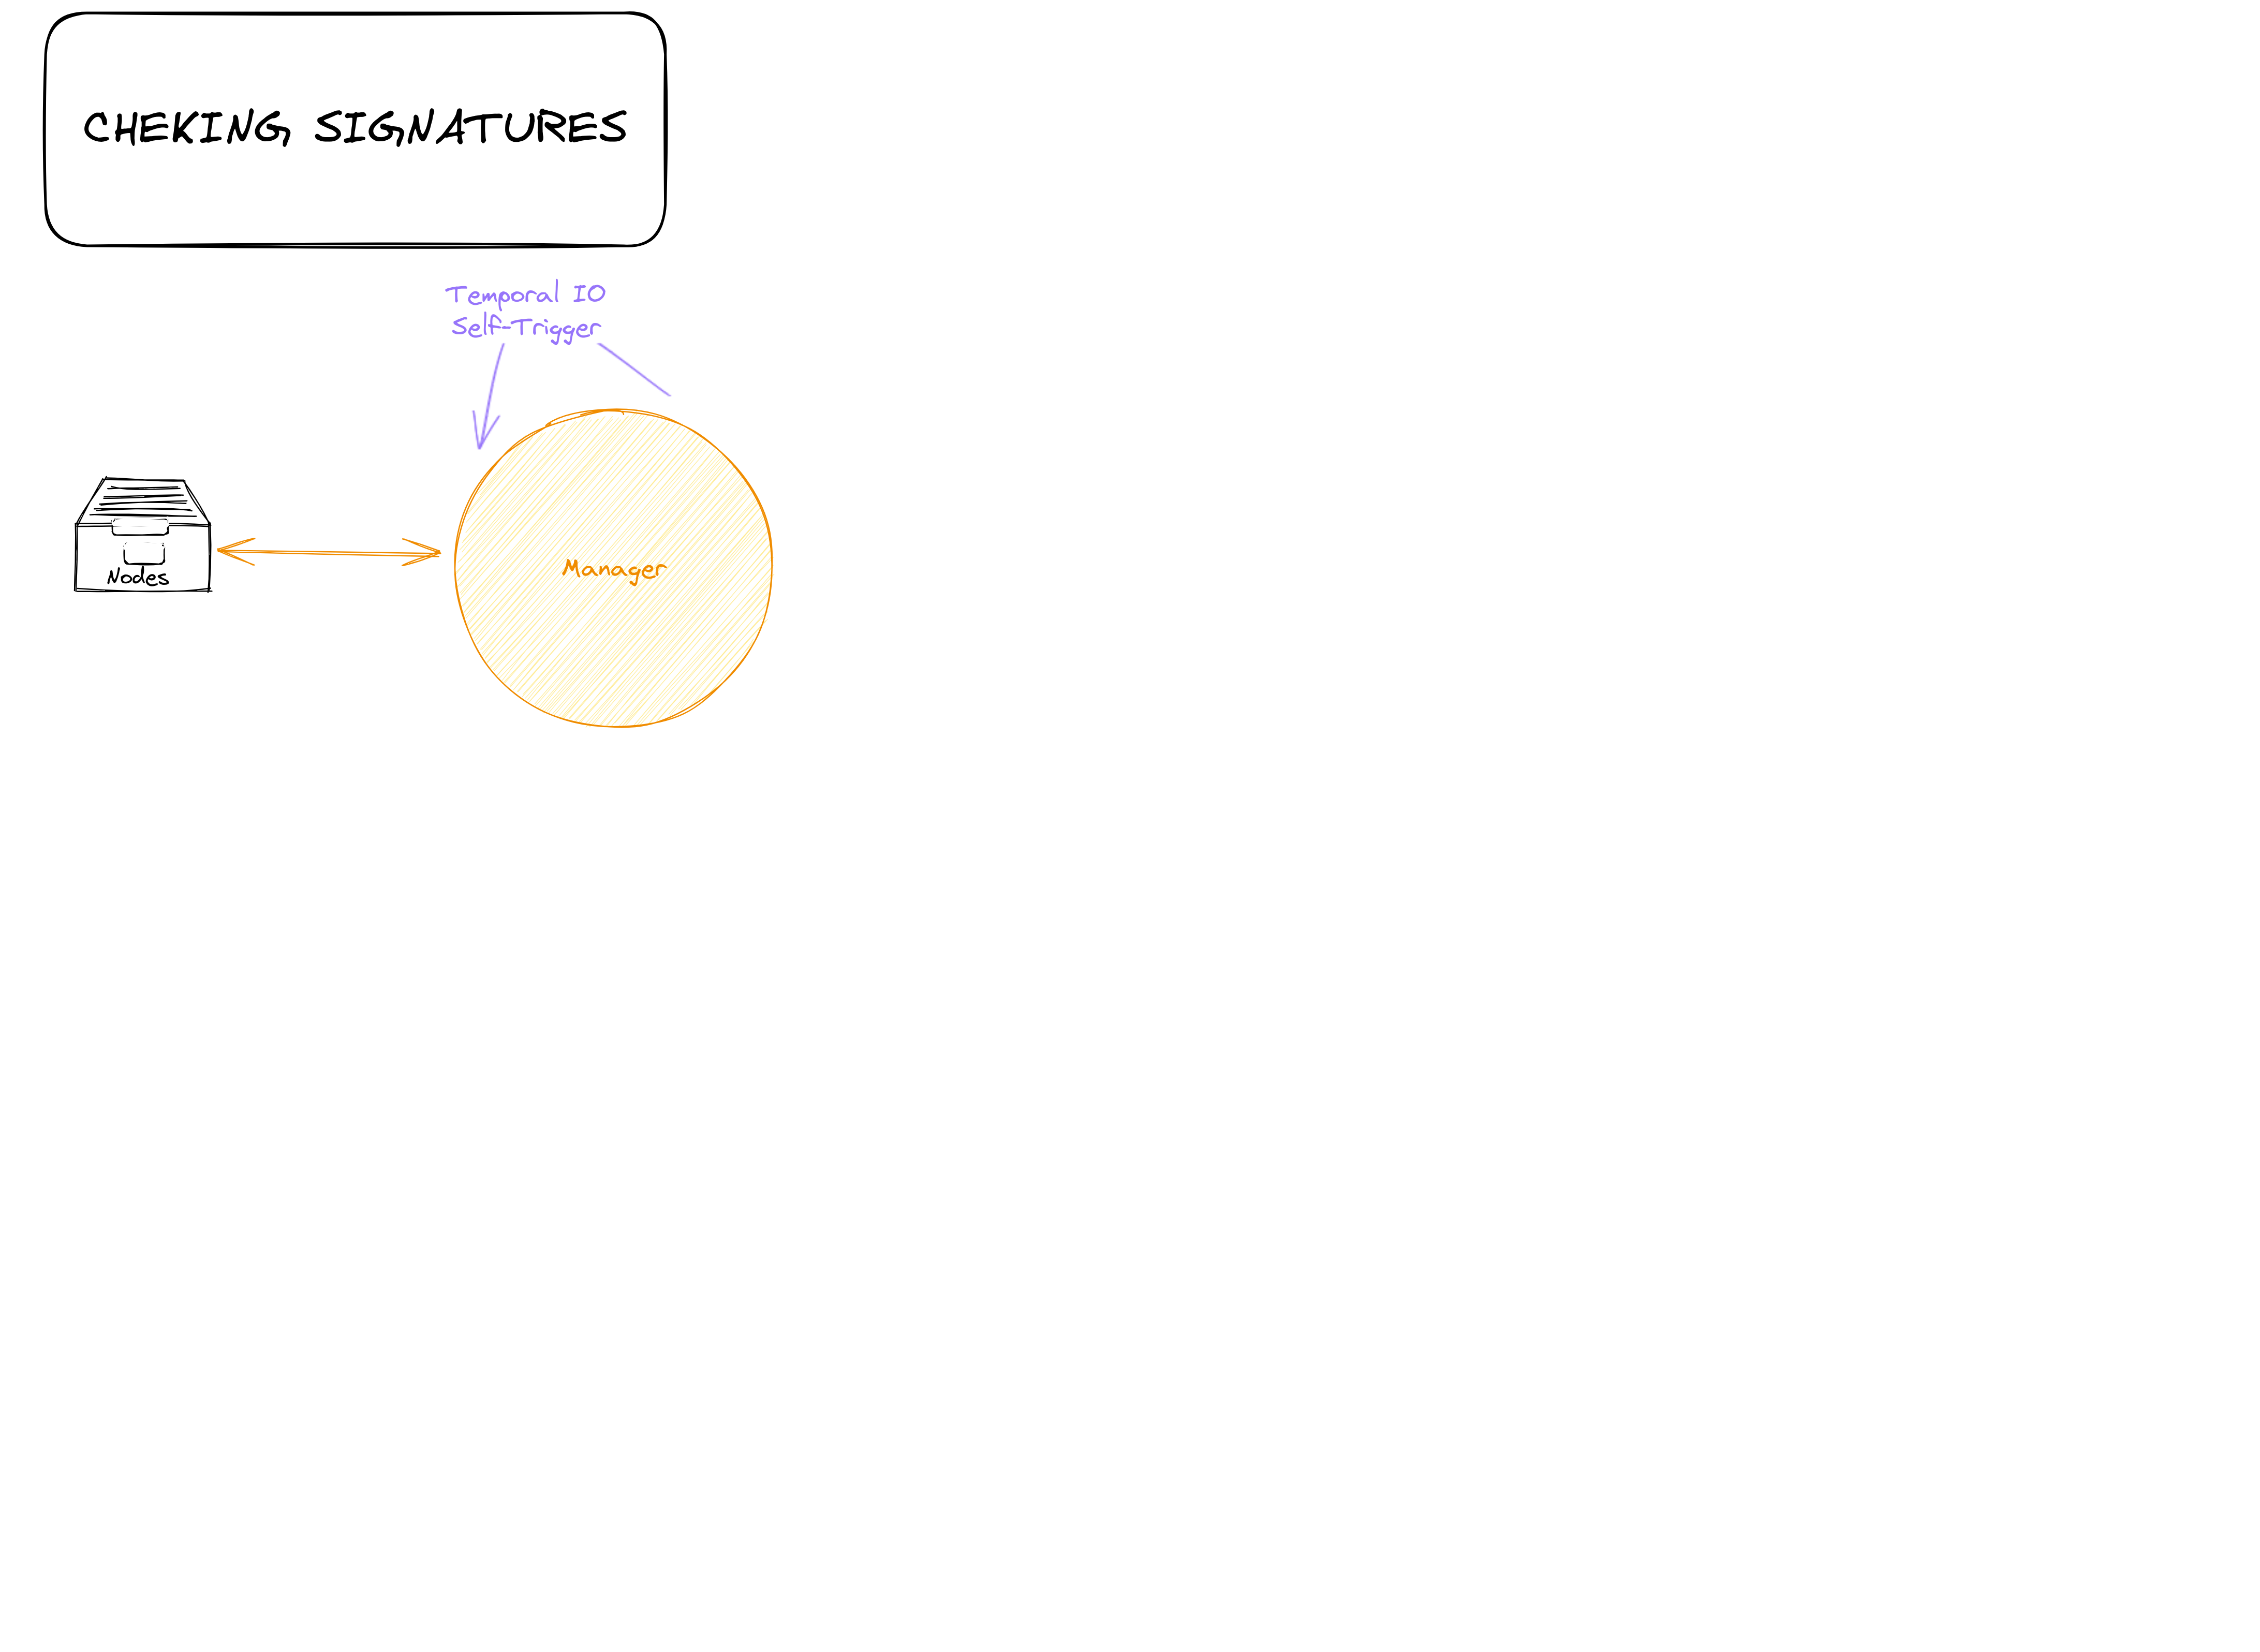
\includegraphics[width=0.8\textwidth]{workflow1}
    \caption{}
    \label{secb:fig:wf1}
\end{figure}

\paragraph{Checking signatures:}
The Manager will check if $N$ in $S$ has a signature $\sigma$ associated in the nodes collection. The signatures are the first thing to check because they are either requirements for other tasks (i.e. tokenizers data) or they signal if a node changed or not (which would trigger complete resampling).

In the particular case of testing \gls{LM}, the most important signature consists of a hash of its tokenizer $T$, hereafter referenced as $\sigma(T)$. 
In ease of expression, we will refer to the signature of node $N$ in $S$ as $\sigma(T_{N}^{S})$. Without a tokenizer signature (signaling that we know the tokenizer) the rest of the tests cannot be performed.
Figure \ref{secb:fig:wf1} shows the workflow until this step.


\begin{figure}[htb!]

    \centering        
    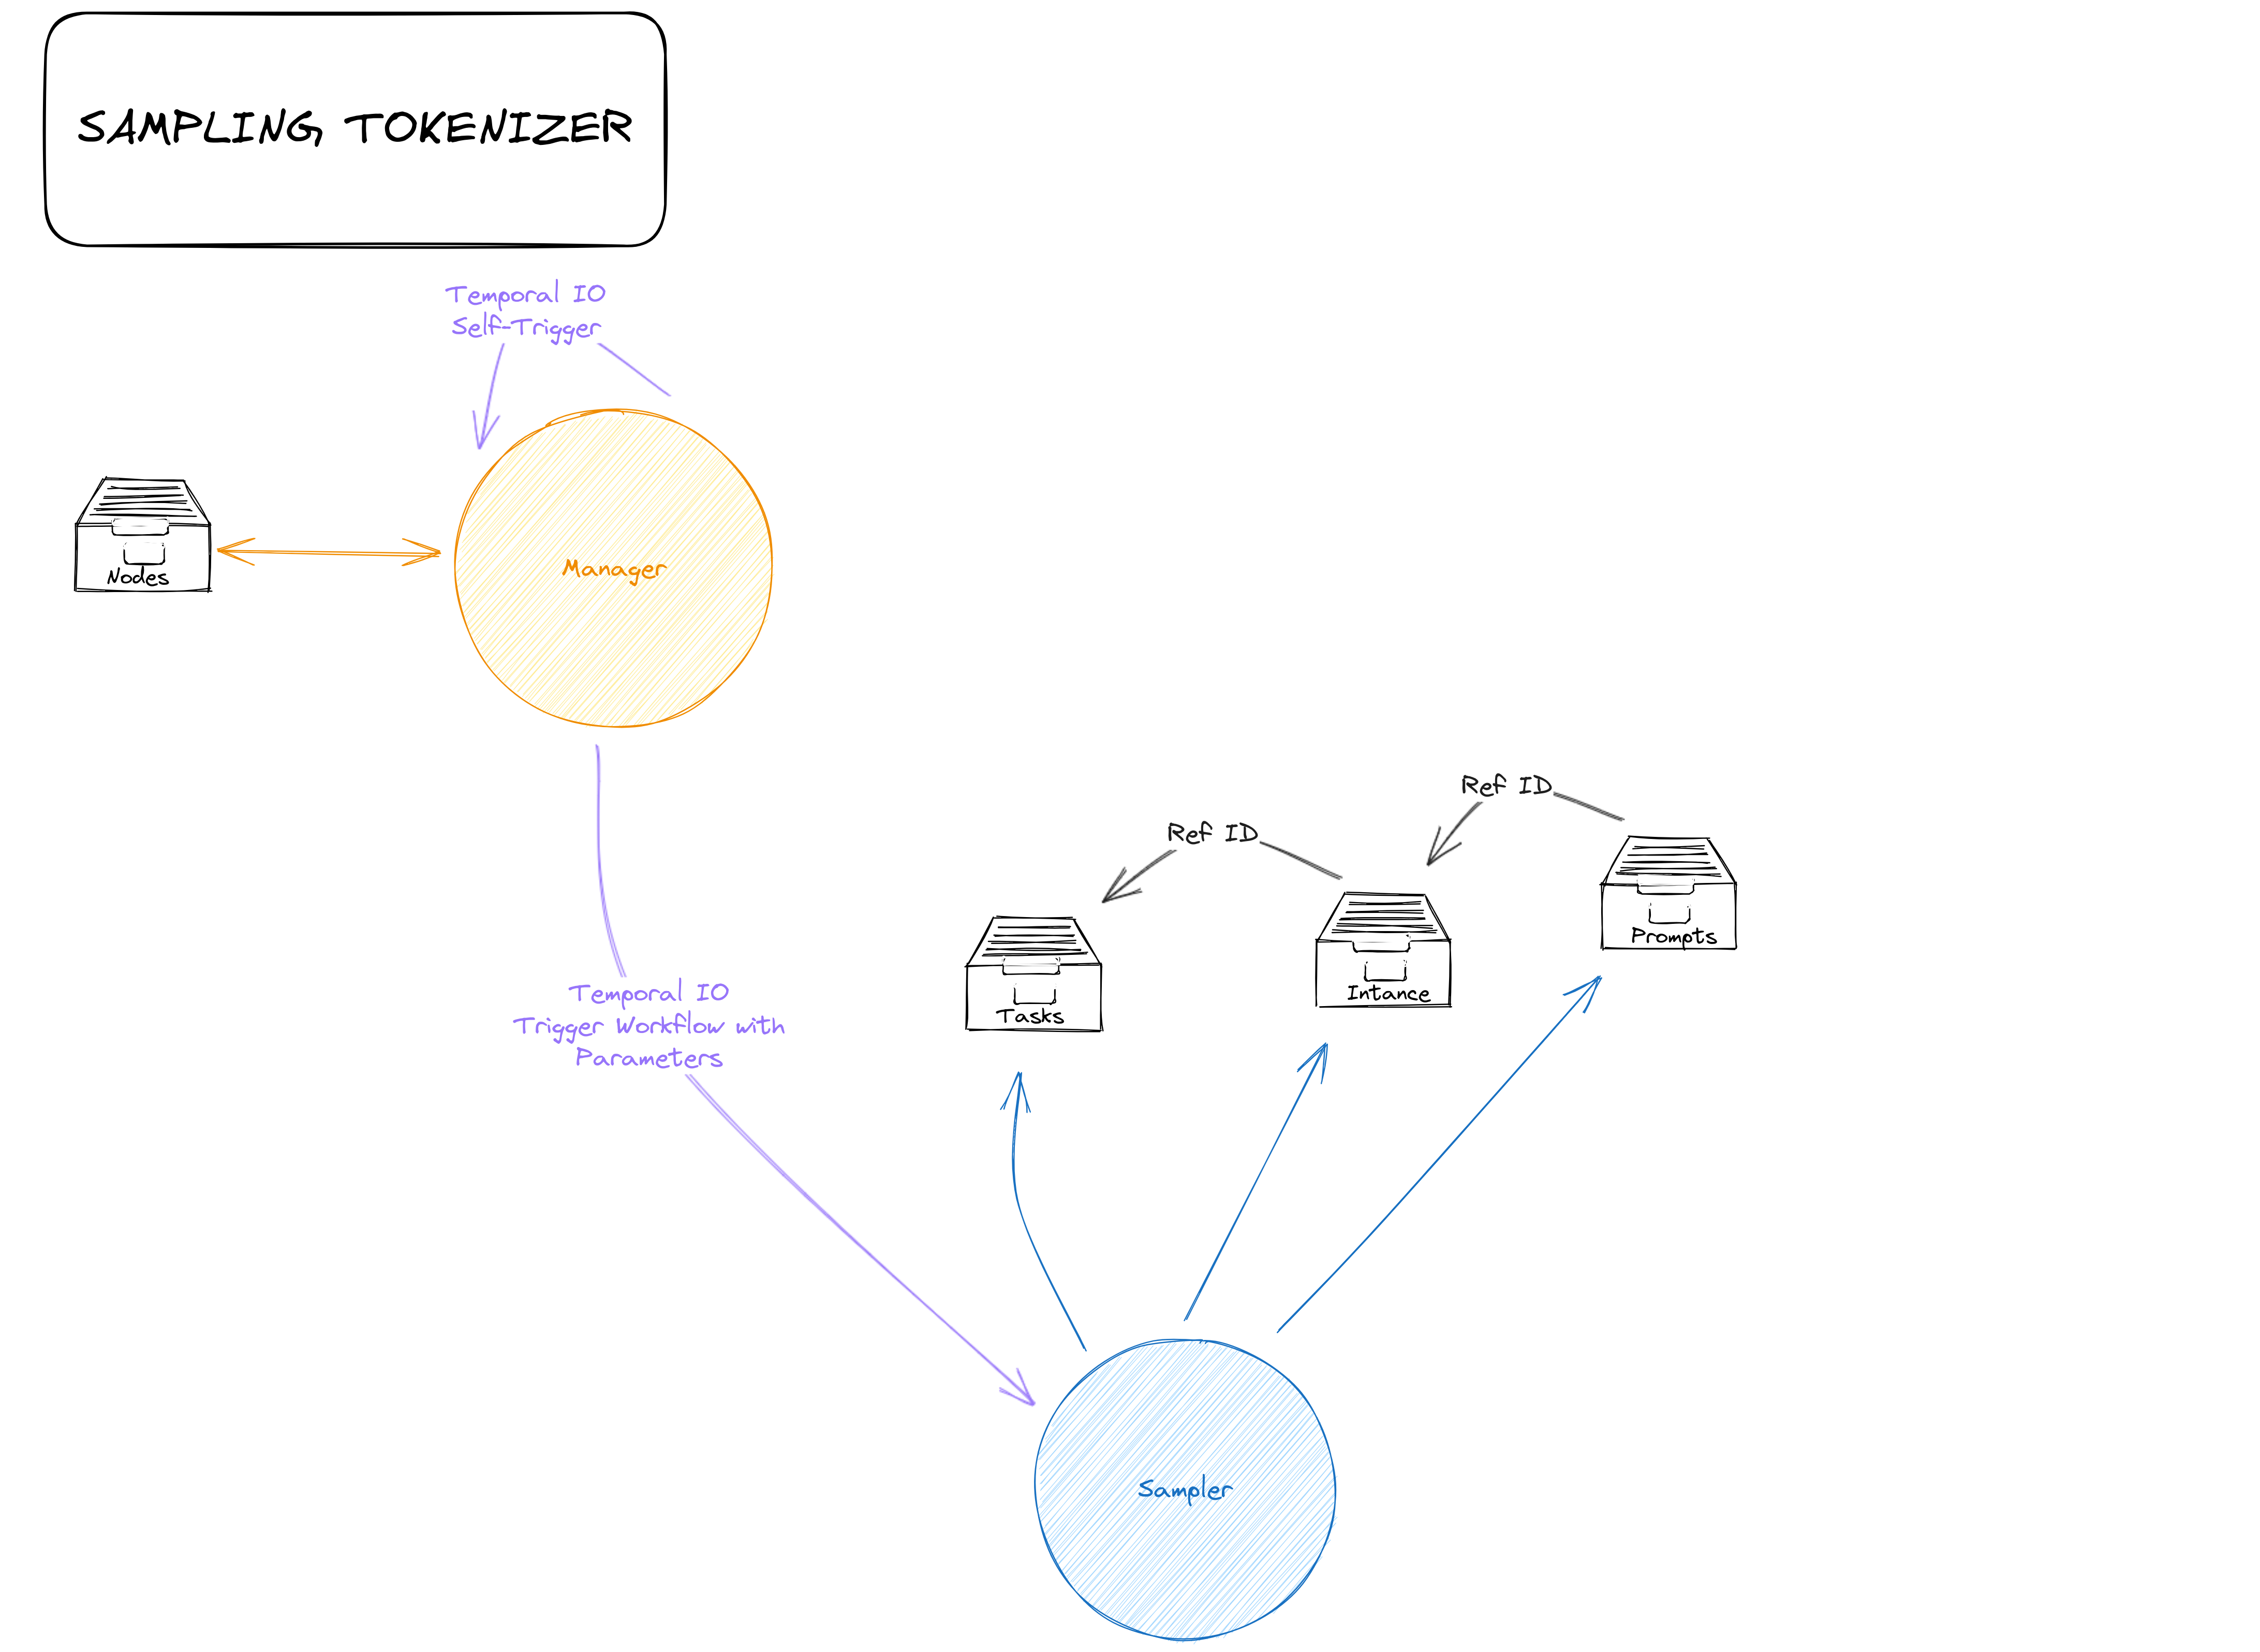
\includegraphics[width=0.8\textwidth]{workflow2}
    \caption{}
    \label{secb:fig:wf2}
\end{figure}



\paragraph{Sample tokenizer:}
To produce the tokenizer signature, the Manager triggers the Sampler module to save a prompt for the Requester pointing to the endpoint of $N_s$ in the \textit{prompts} collection.
Figure \ref{secb:fig:wf2} shows the workflow until this step.



\begin{figure}[htb!]
    \centering        
    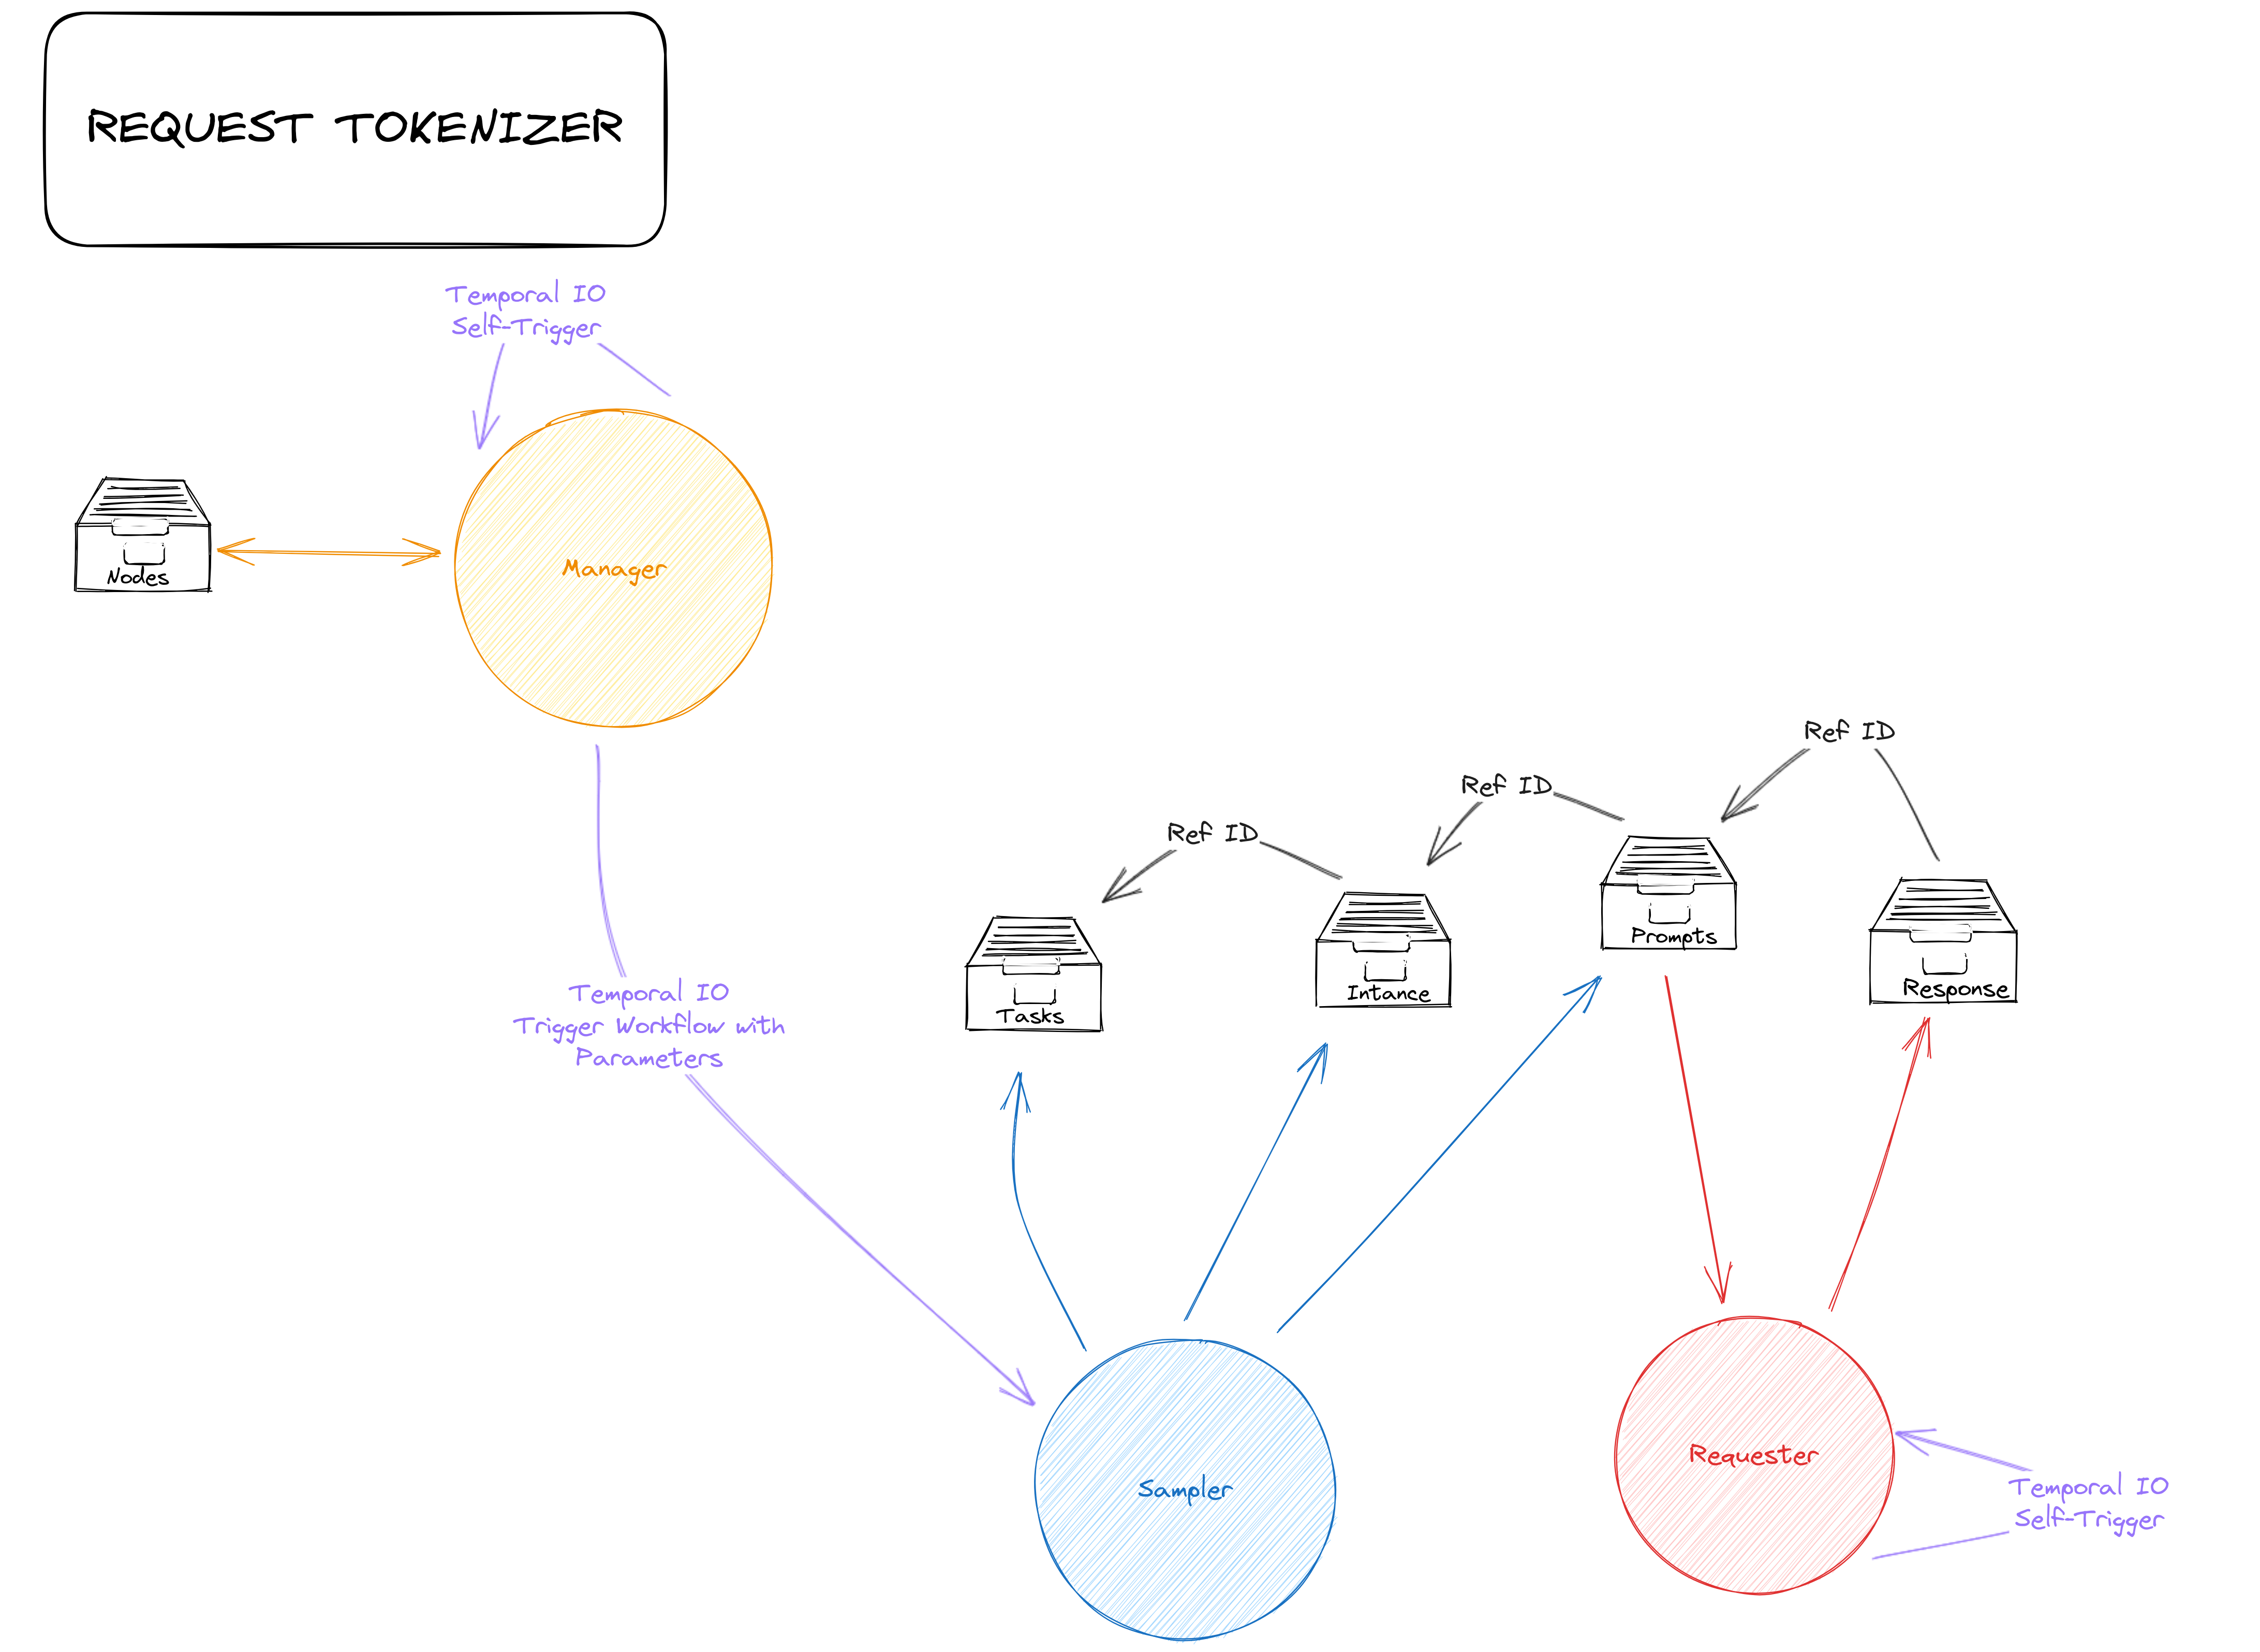
\includegraphics[width=0.8\textwidth]{workflow3}
    \caption{}
    \label{secb:fig:wf3}
\end{figure}


\paragraph{Request tokenizer:}
The tokenizer signature, is produced from the a full json tokenizer $T$ data that is available in the \emph{pokt/tokenizer} endpoint of the POKT Sidecar. This prompt is not responded by the OpenAI API because it is not part of the spec since the tokenizer is known. In the case of the POKT network, the tokenizer is unknown because the model itself is unknown.
Figure \ref{secb:fig:wf3} shows the workflow until this step.


\begin{figure}[htb!]
    \centering        
    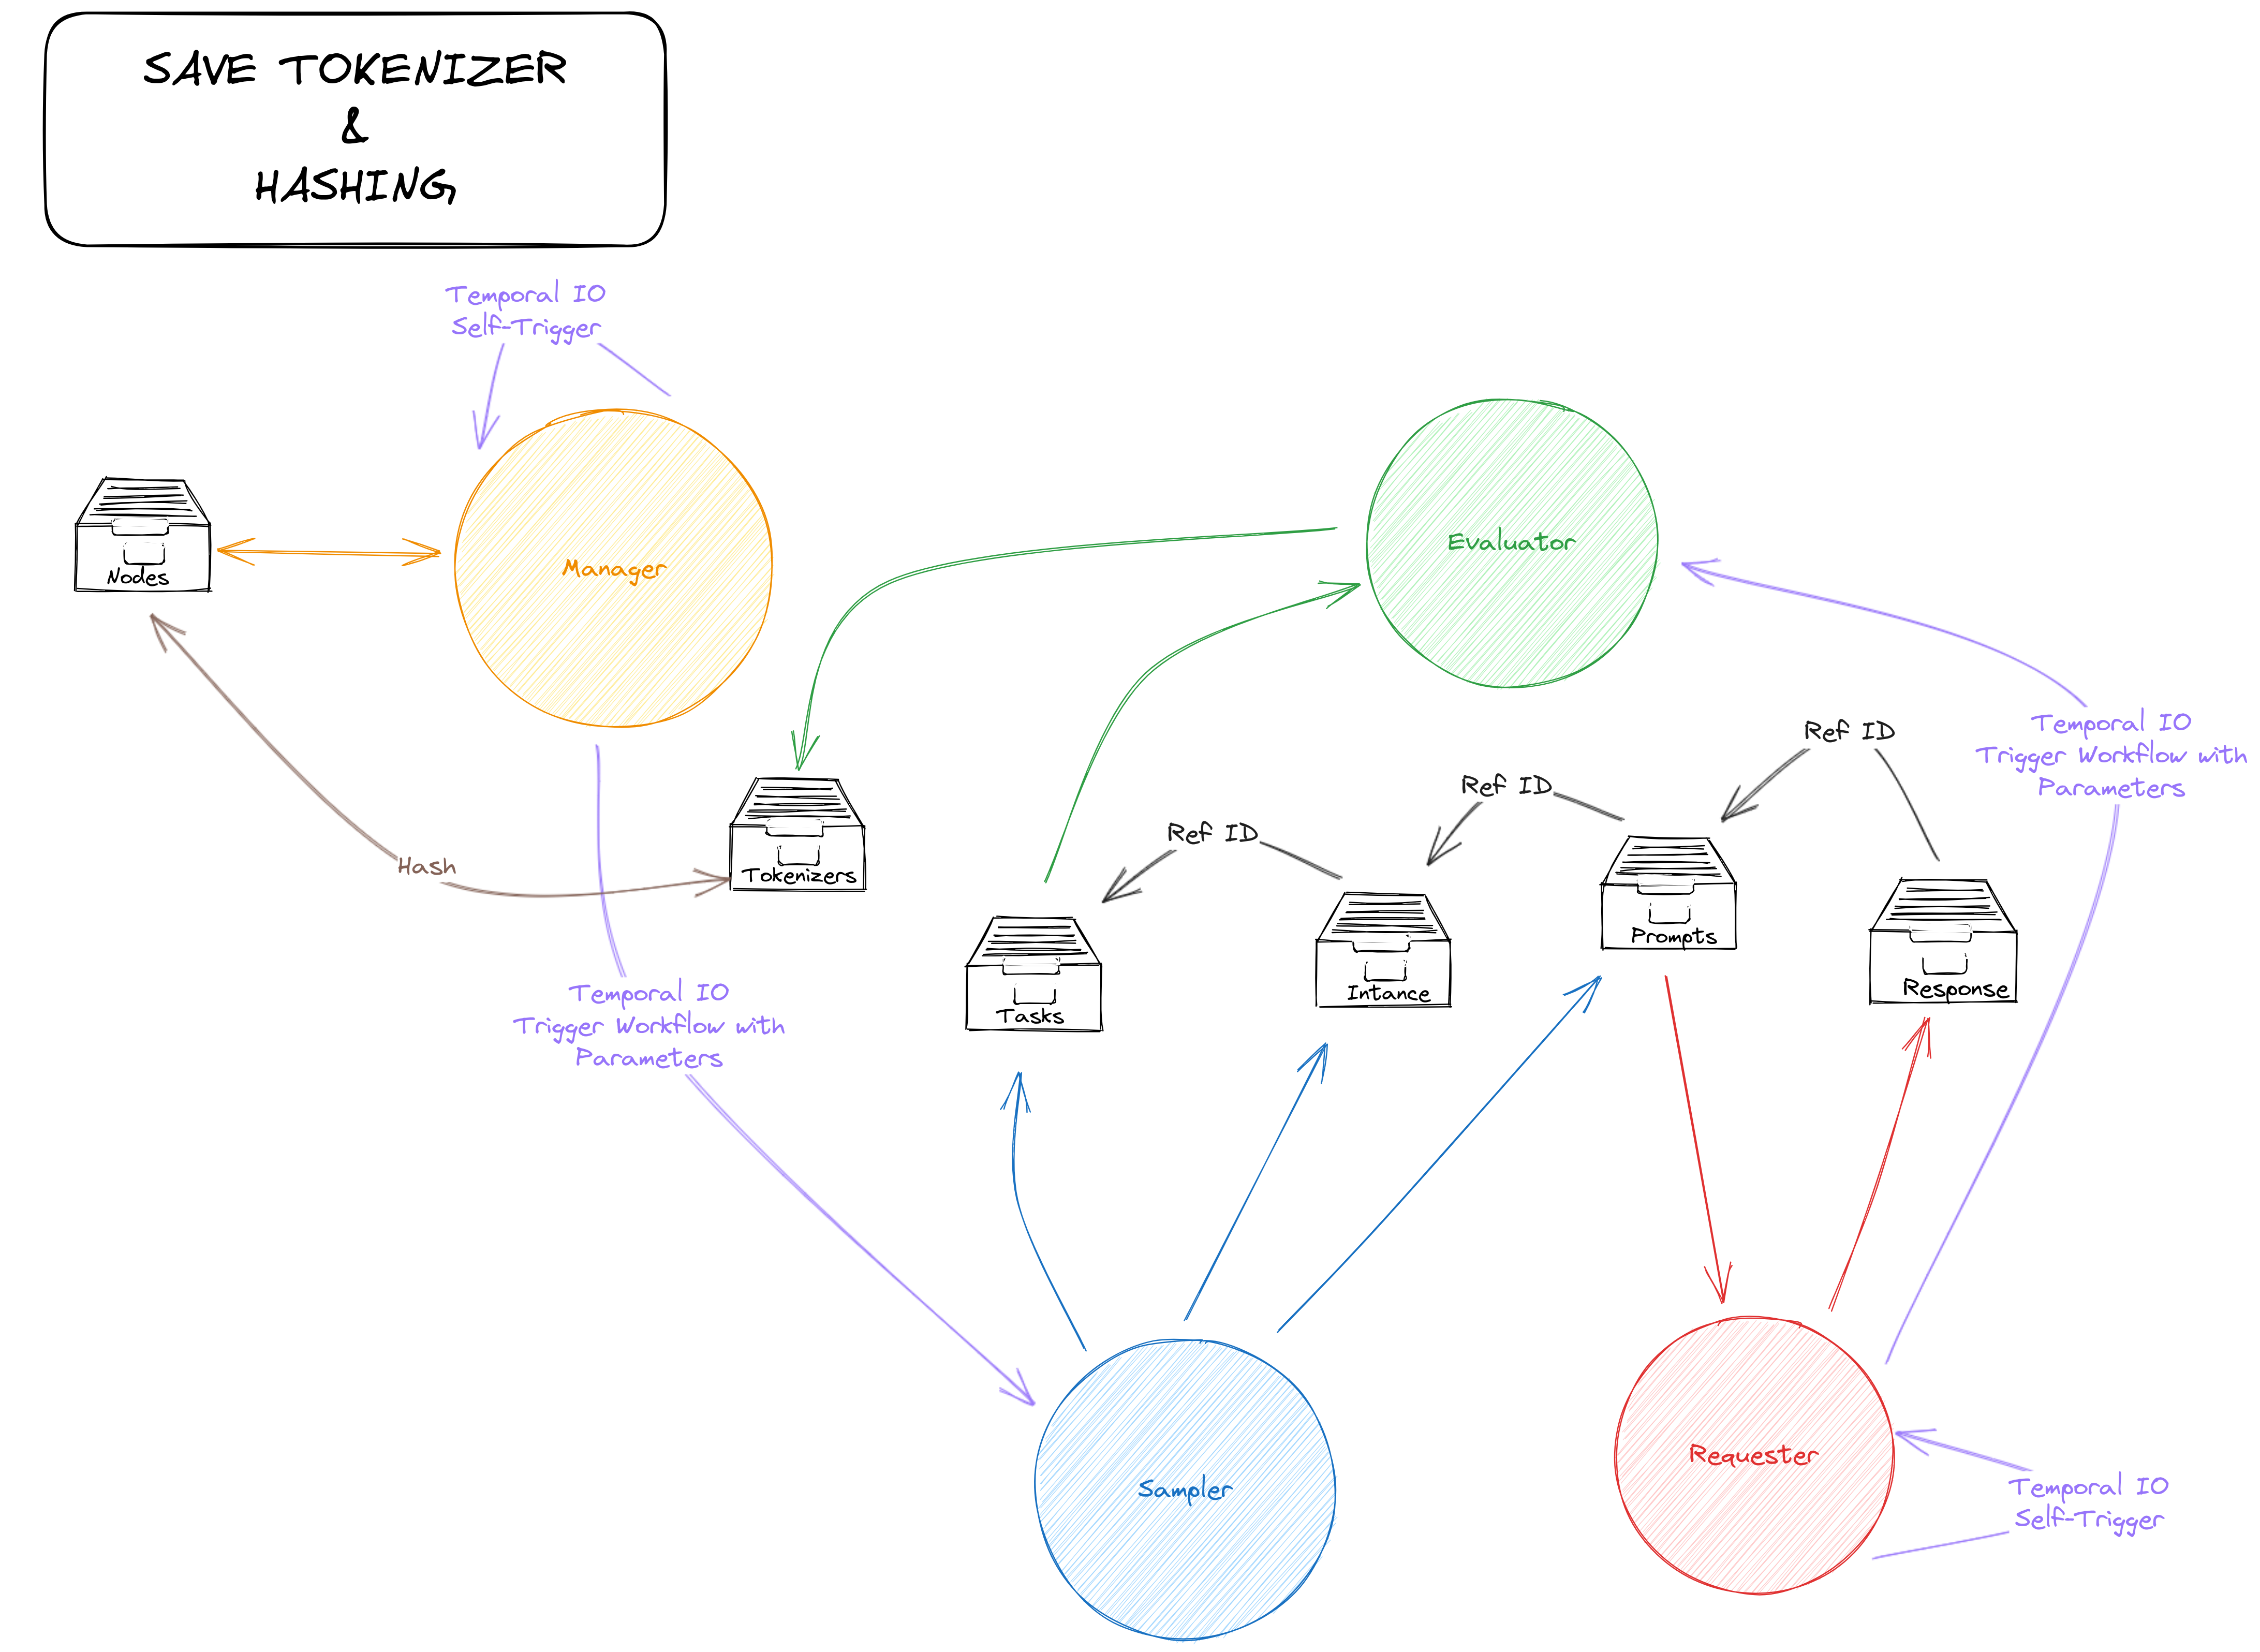
\includegraphics[width=0.8\textwidth]{workflow4}
    \caption{}
    \label{secb:fig:wf4}
\end{figure}


\paragraph{Save tokenizer:}
Finally the evaluator loads the Requester response and calculates the tokenizer hash. If the tokenizer is not already tracked in the tokenizers collection, it will create a new entry. Finally the Manager will recover the tokenizer hash from the results collection entry and add it to the node data. Figure \ref{secb:fig:wf4} shows the workflow until this step.

\begin{figure}[htb!]
    \centering
    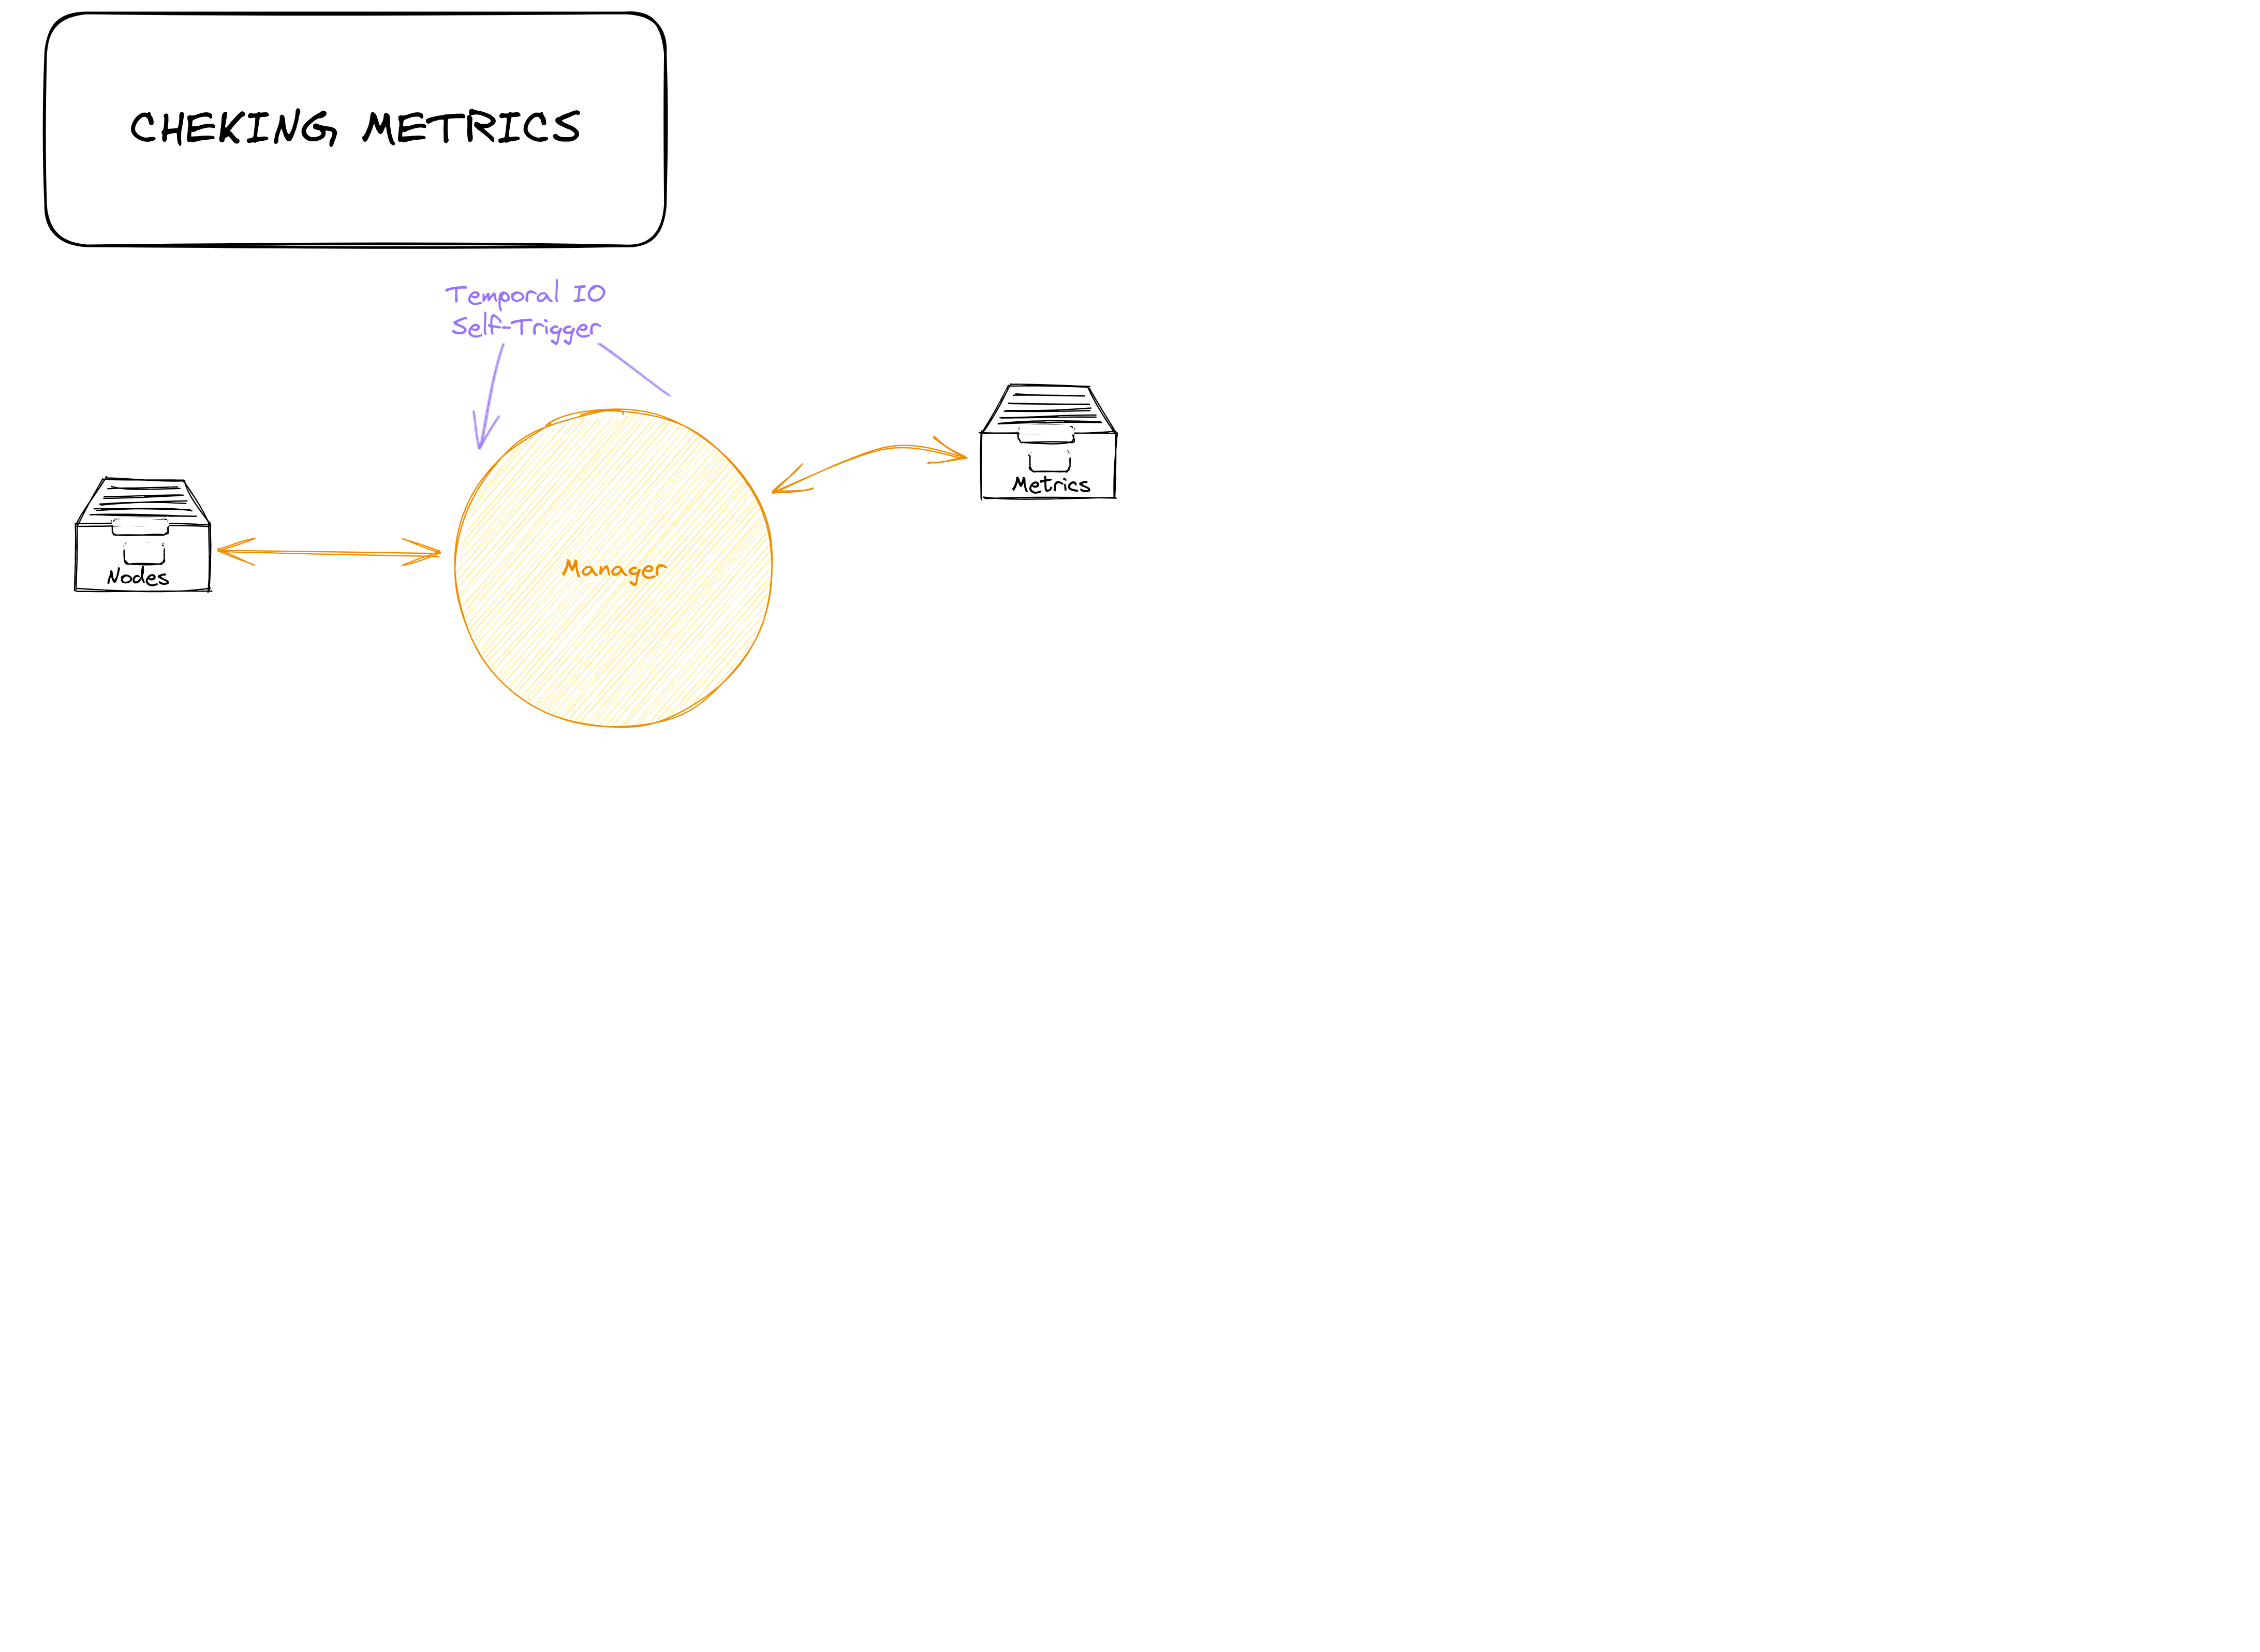
\includegraphics[width=0.8\textwidth]{workflow5}
    \caption{}
    \label{secb:fig:wf5}
\end{figure}


\paragraph{Checking metrics:}
Once a node has its signature, the Manager will check if any sample related to a metric of a task needs to be updated, either because the configured time has expired, or it does not yet have a sufficient number of samples to produce reliable metrics. 
If required, the Manager will trigger the Sampler, requiring from the Sampler a quantity $q$ of samples for the task. 
Figure \ref{secb:fig:wf5} shows the workflow until this step.


\begin{figure}[htb!]
    \centering
    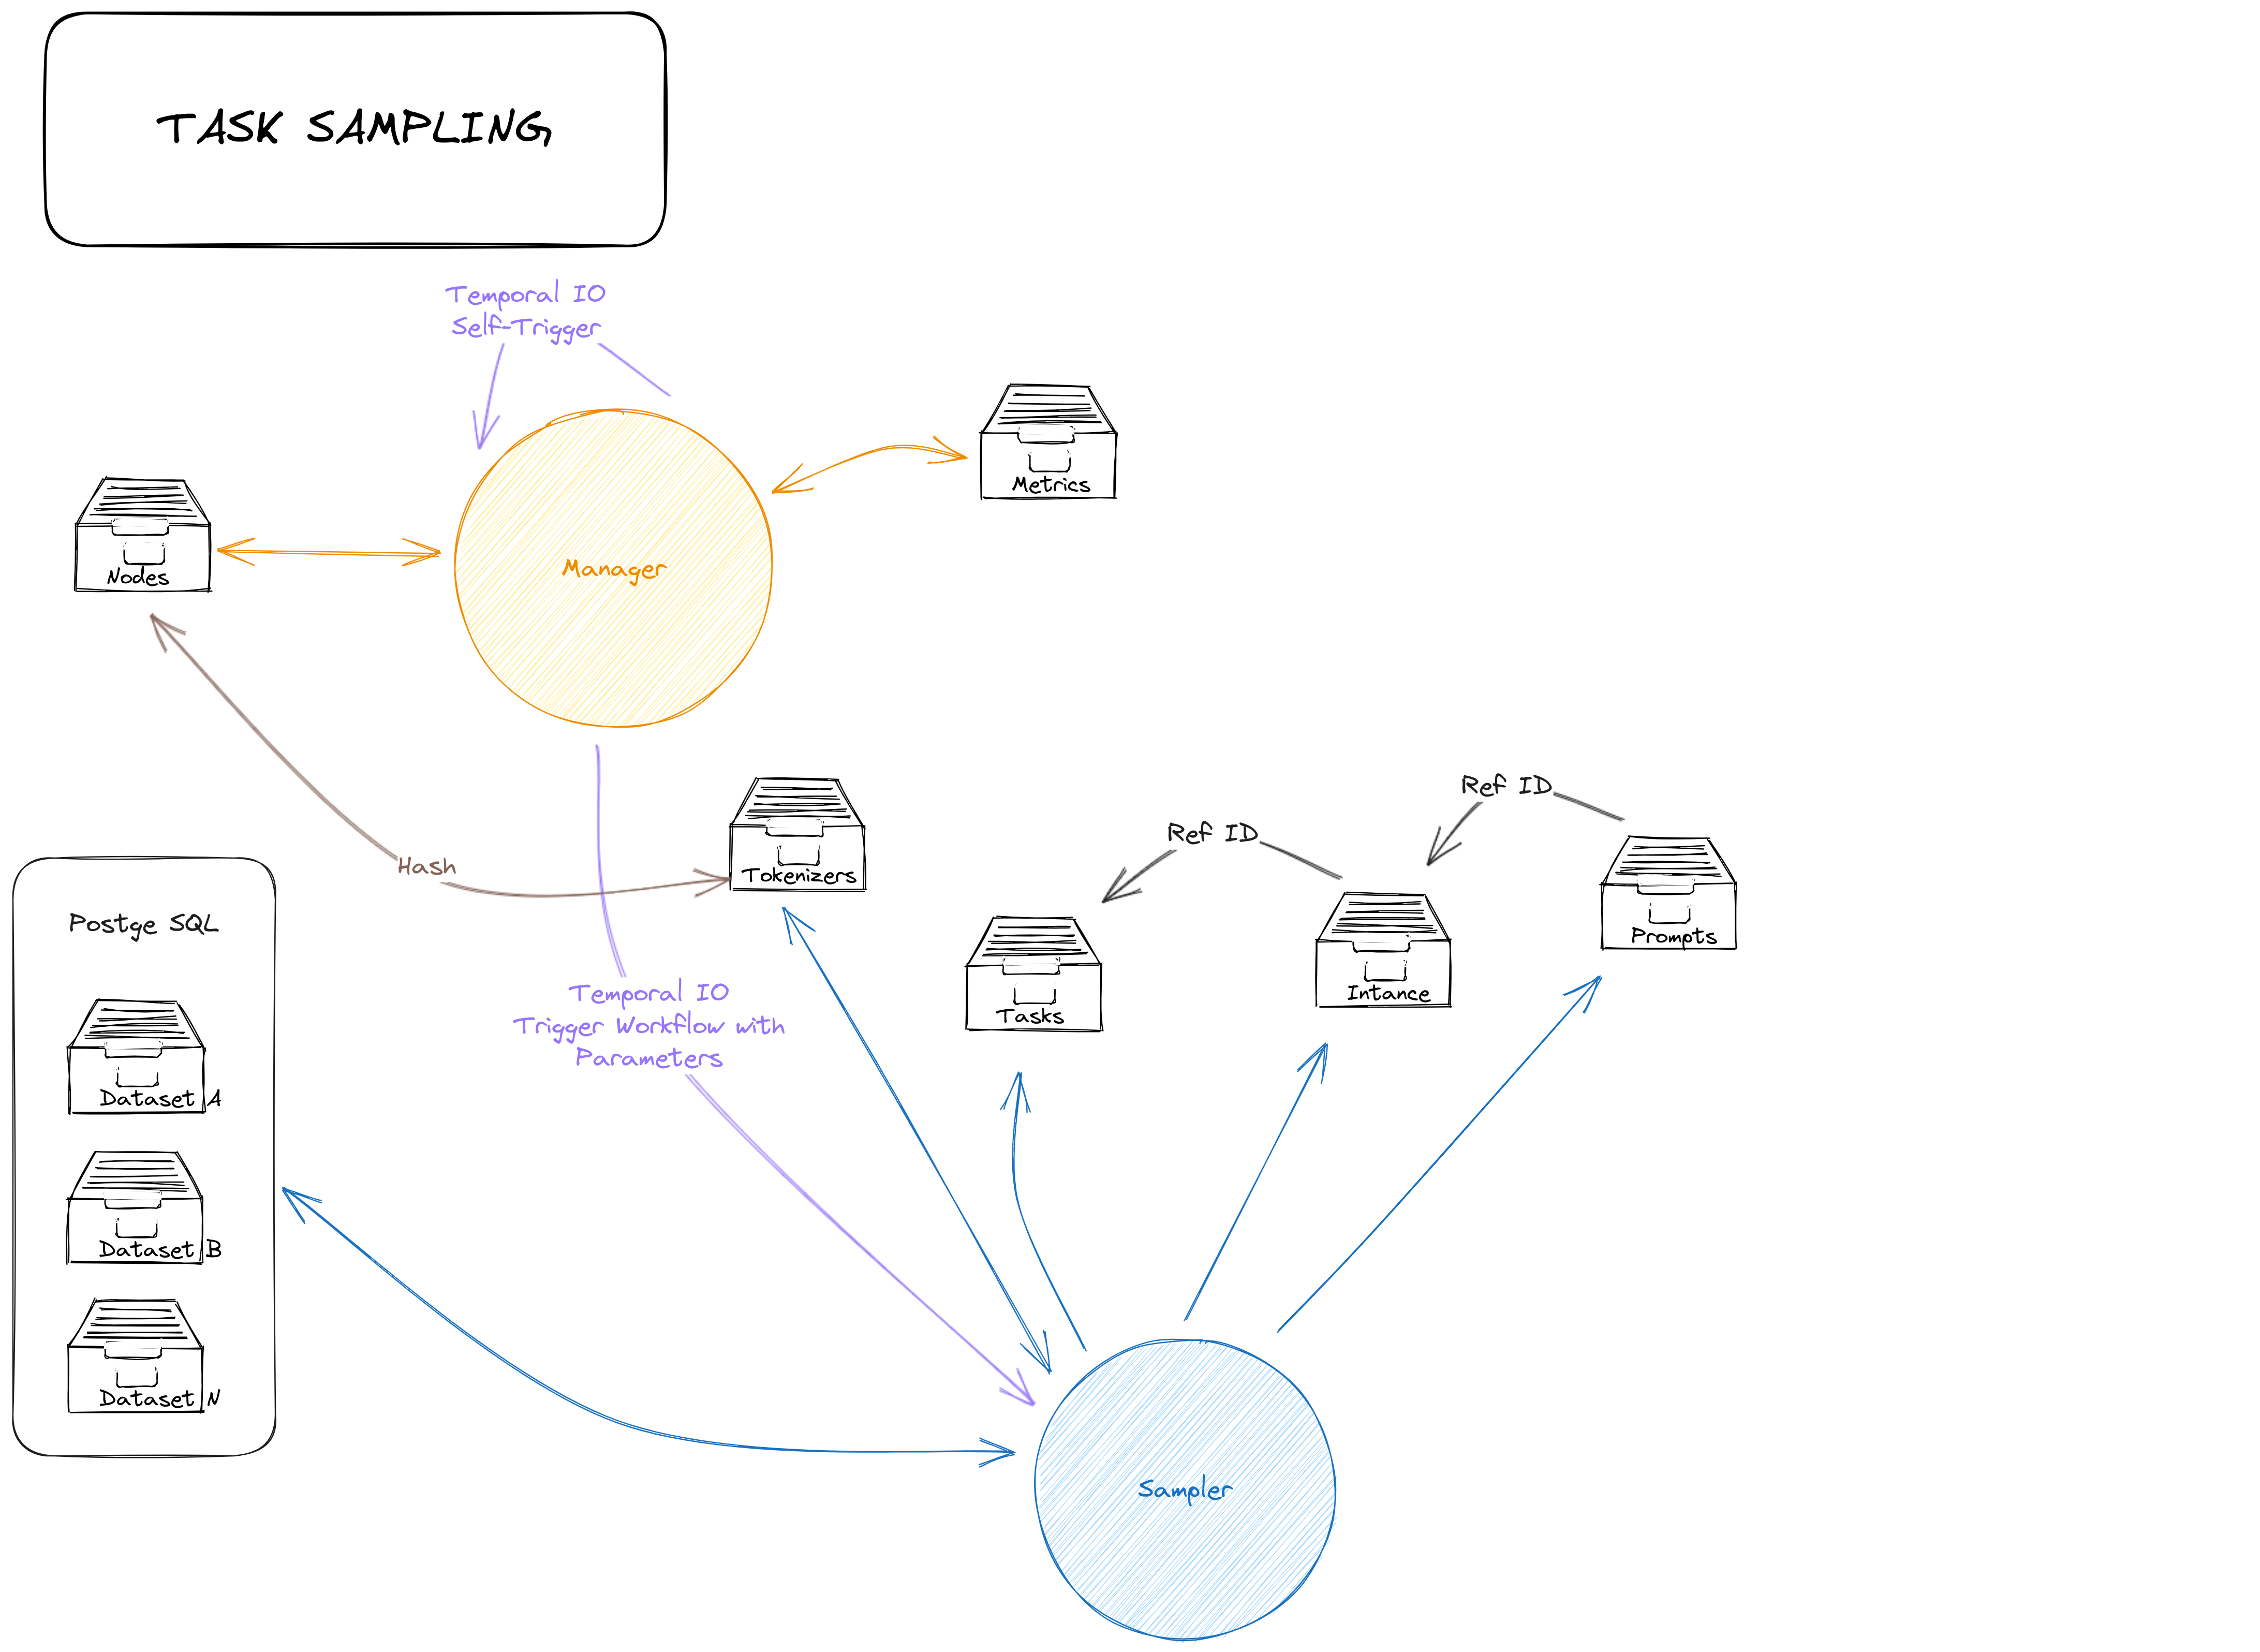
\includegraphics[width=0.8\textwidth]{workflow6}
    \caption{}
    \label{secb:fig:wf6}
\end{figure}

\paragraph{Task sapling:}
When the Sampler receives the request from the Manager, it will load the dataset corresponding to the task but avoiding to load samples previously requested from the evaluation dataset. 
The Sampler randomly selects $q$ docs from the dataset, and create a \gls{LM} prompt following the OpenAI API. The Sampler ends by saving the task, instance, prompt and request information the corresponding collections.
Figure \ref{secb:fig:wf6} shows the workflow until this step.

\begin{figure}[htb!]
    \centering
    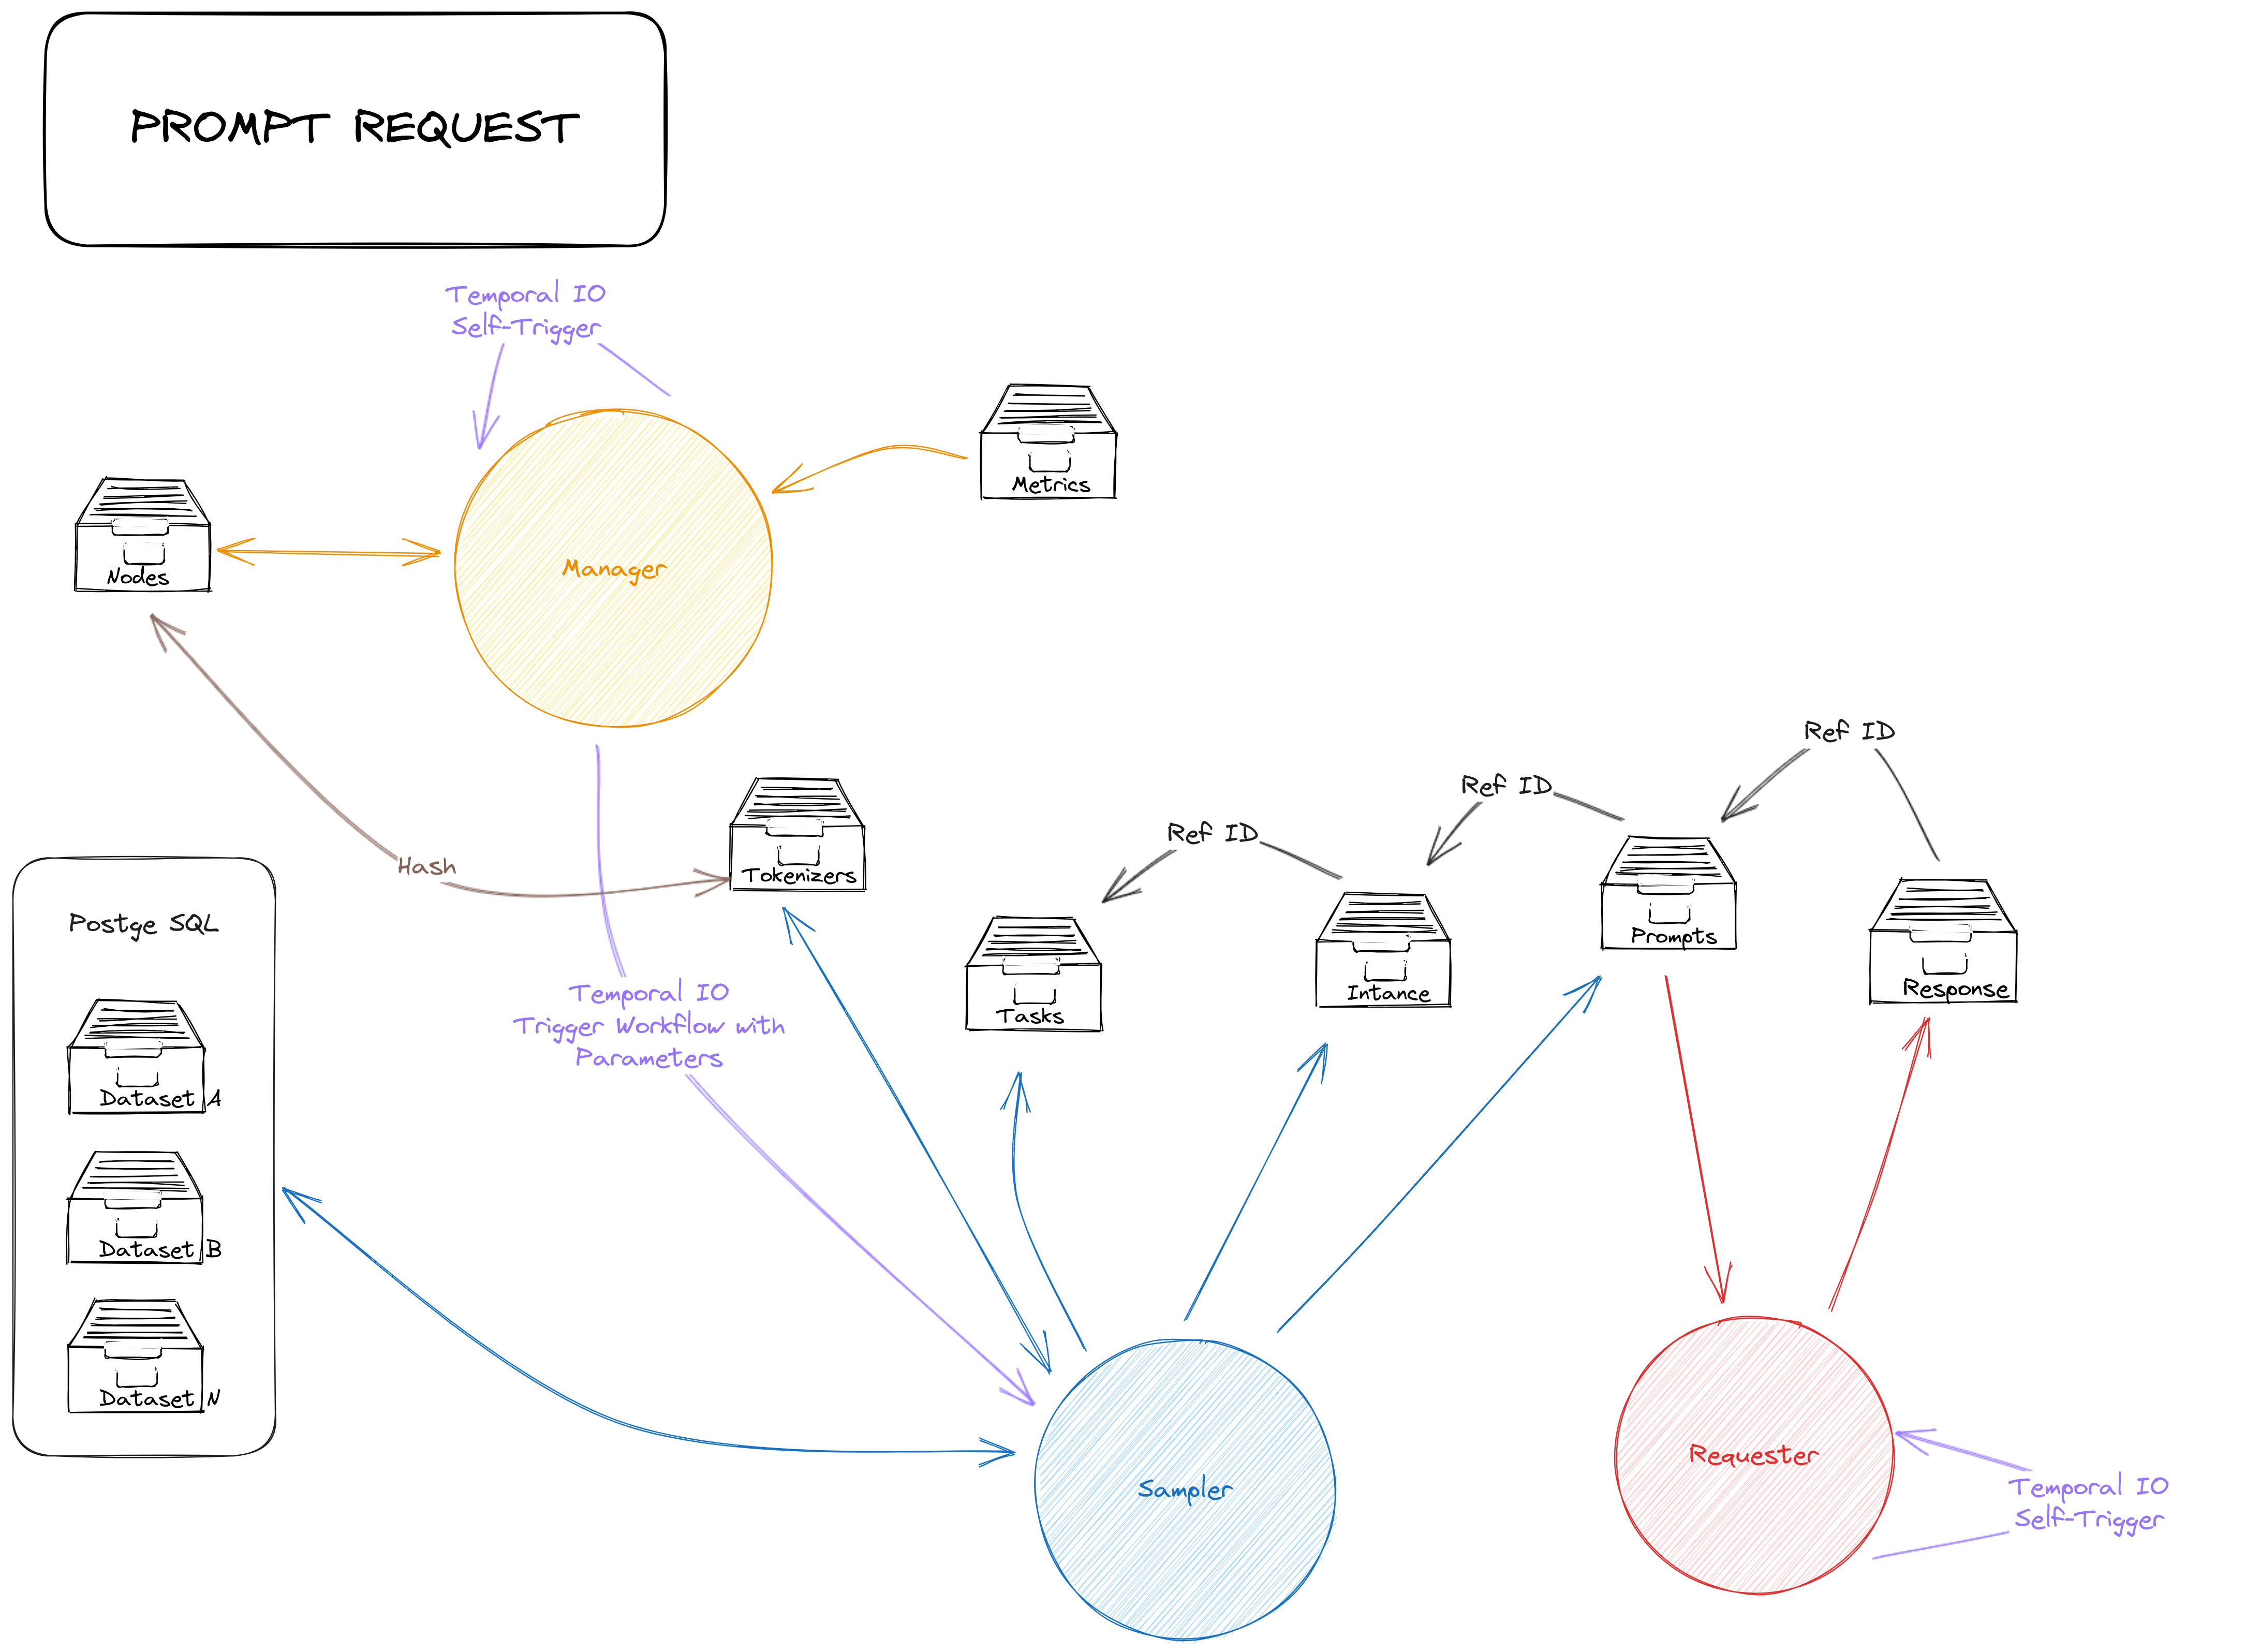
\includegraphics[width=0.8\textwidth]{workflow7}
    \caption{}
    \label{secb:fig:wf7}
\end{figure}


\paragraph{Prompt request:}
After the asynchronous creation of the request by the Sampler, the Requester will try to prompt the node whenever it enters into session with one of its controlled apps. It is normal that the task will remain in the collection for a long period until this happens. Once the requested node is found in session, the relay is done and the result is written to the response collection.
Figure \ref{secb:fig:wf7} shows the workflow until this step.

\begin{figure}[htb!]
    \centering
    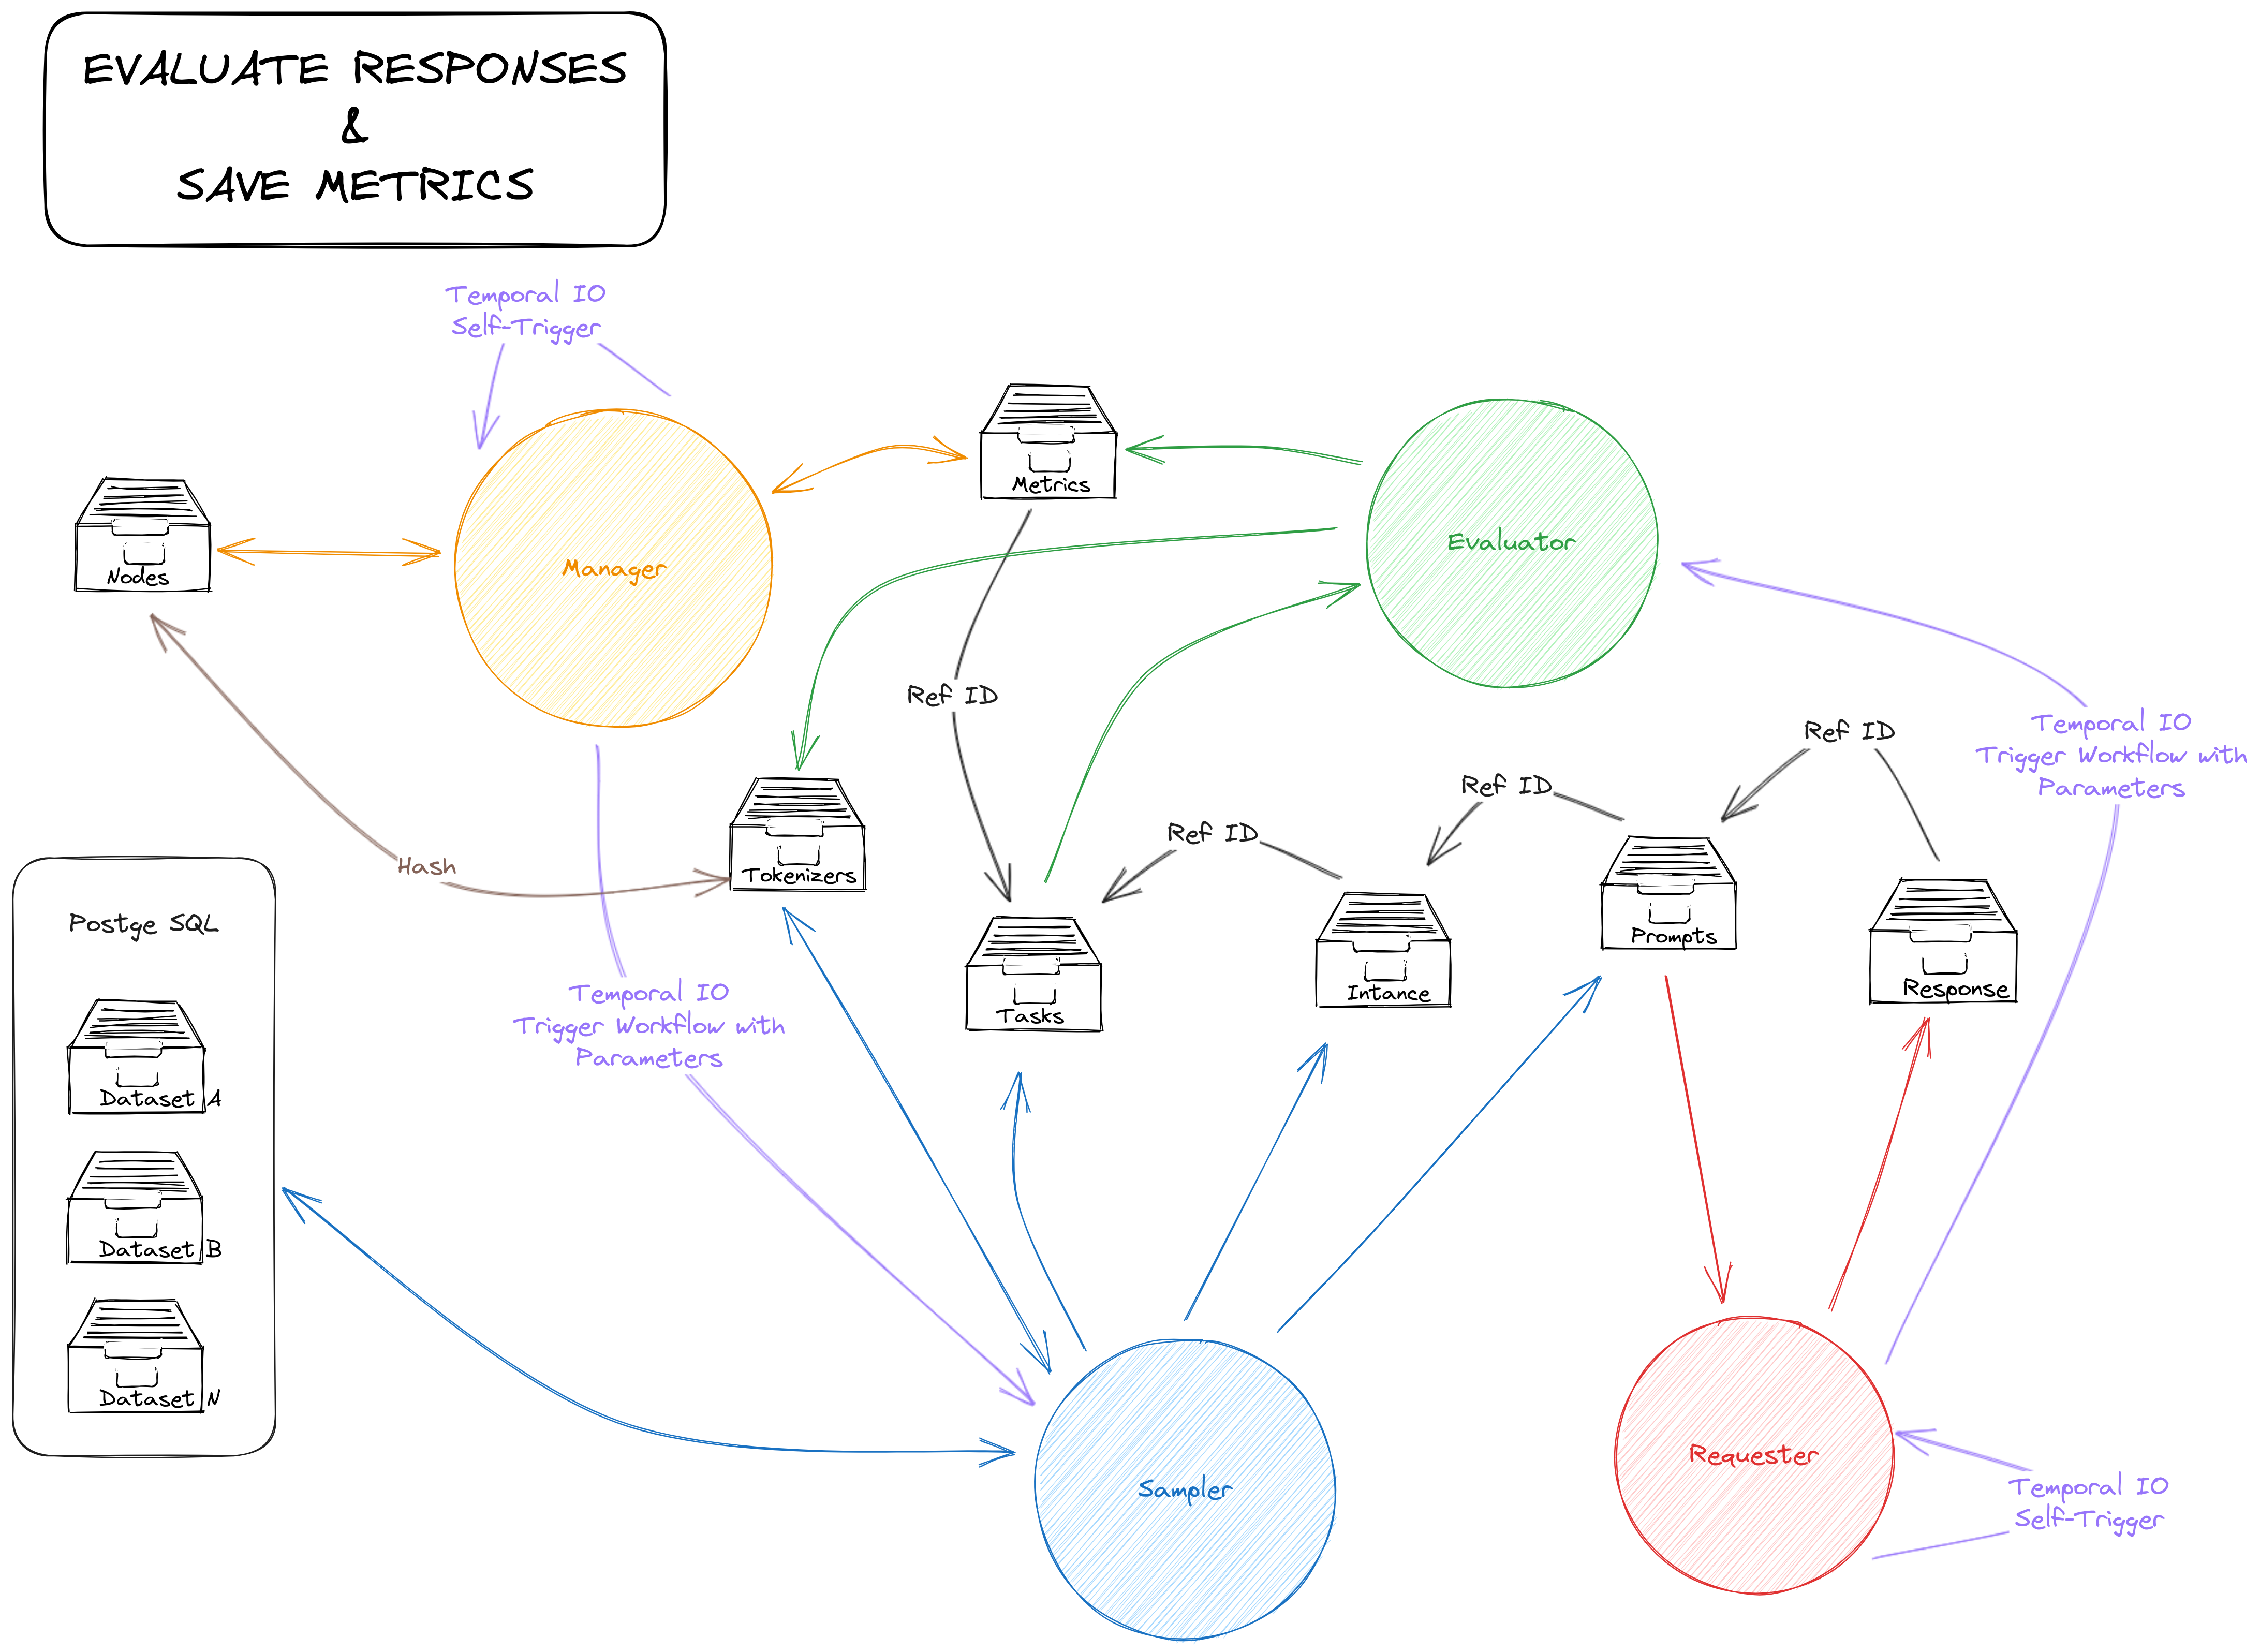
\includegraphics[width=0.8\textwidth]{workflow8}
    \caption{}
    \label{secb:fig:wf8}
\end{figure}

\paragraph{Evaluation response \& save metrics:}
The Evaluator can be triggered by the Requester when a task is marked as done, meaning that all request had been responded, or by a periodic time previously configured. 
At this point it is necessary to regenerate the same evaluation state as if lm-eval-harness had been executed locally, that is to say, the same execution state is generated (this includes: task, instance, prompt, datasets, etc) as the Sampler, with the addition that now we have the responses. 
It is important to mention that because Requester simply returns any response that the Pocket Network node sends it, and this includes any type of error, the Evaluator will only be able to continue with the evaluation and generate metrics when at least one sample has all its requests responded. 
To recall, the relation between a sample and requests is 1:N, as was illustrated in the previous report. 
Figure \ref{secb:fig:wf8} shows the workflow until this step.



\begin{figure}[htb!]
    \centering
    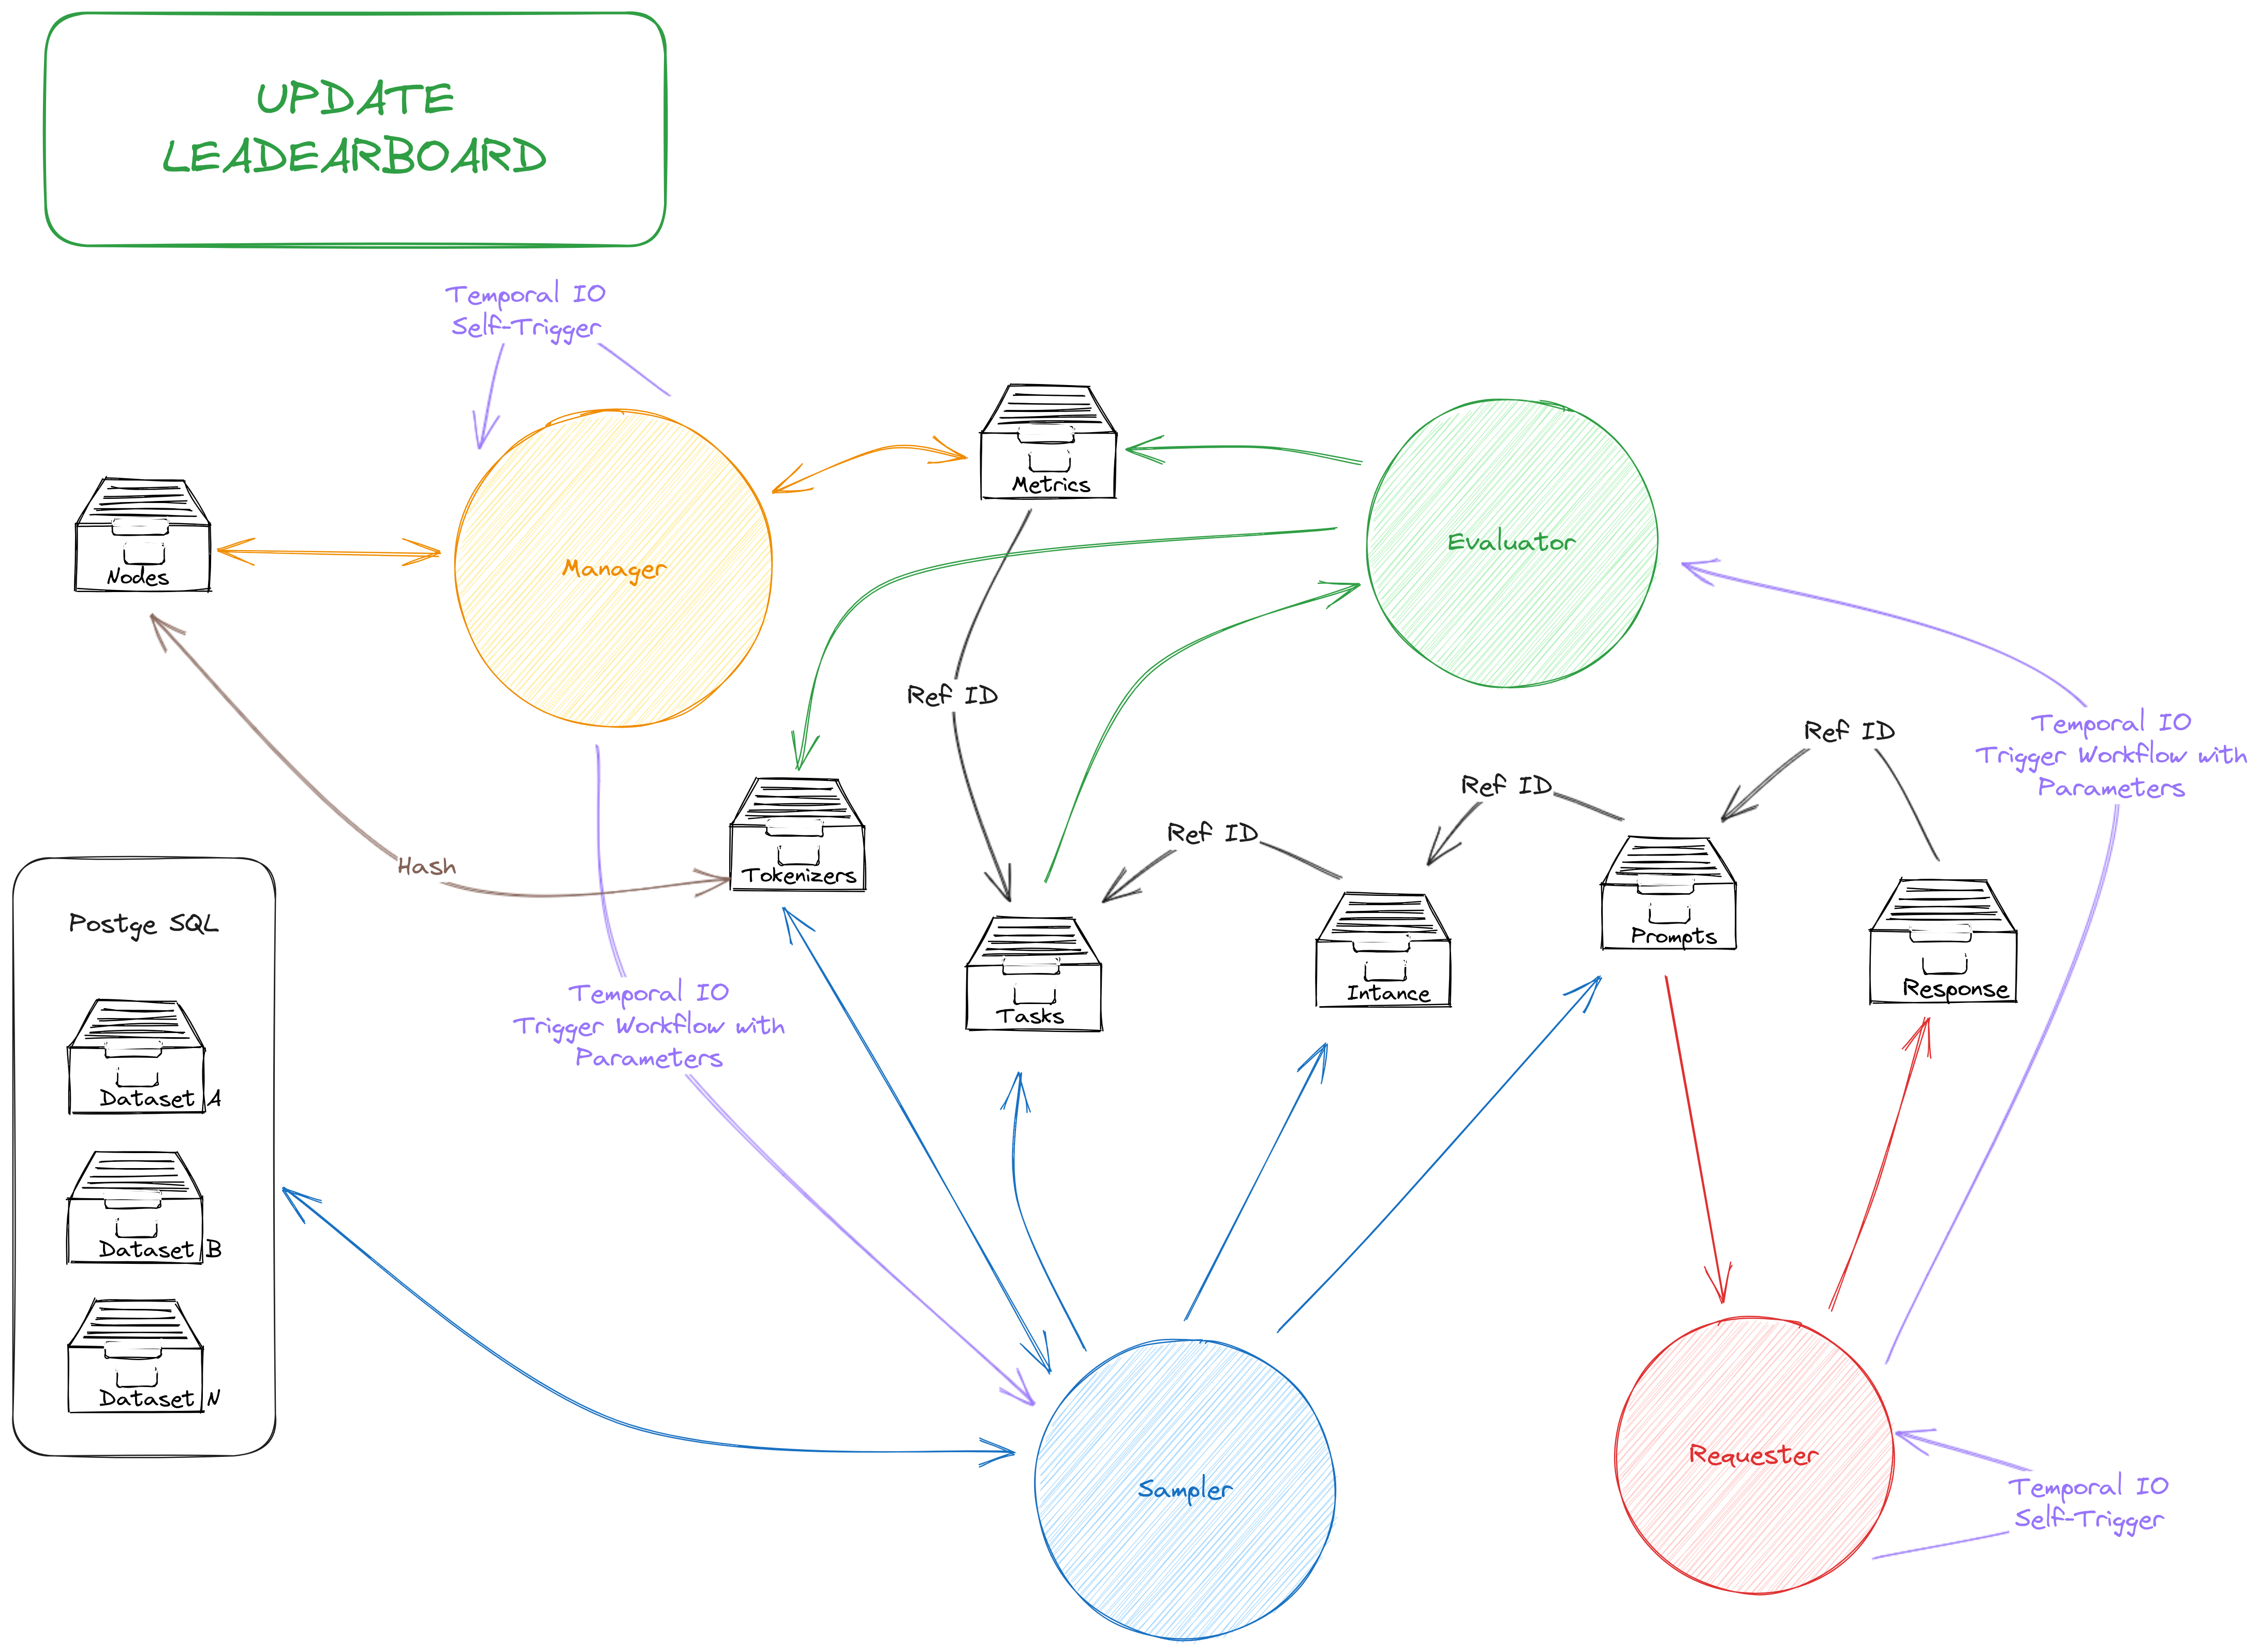
\includegraphics[width=0.8\textwidth]{workflow9}
    \caption{Update metrics.}
    \label{secb:fig:wf9}
\end{figure}

\paragraph{Leaderboard Update:}

Finally, after the Manager has written all the metrics data in the corresponding nodes collections, the API process will re-process the higher level information, such as the leaderboard scores. 
Figure \ref{secb:fig:wf9} shows the last step of the workflow.


% Que quisiste decir aca ameooooo
% Manager detect nodes staked, checking signatures for example tokenizers. If the node has not a signature/tokenizer associated, it will be requested. 
% If signatures are ok, then it will check if the model requires new samples to update any task/metrics. 
% when is required (low threshold of the samples required), trigger sampler. 
% During the creation of the samples, the tokenizer is called, and prepare the prompt. 
% The requester check if there is any prompt not done, and send to trhougth the network. 
% Once each sample from a task is done, the requester marks the task as done. 
% Due to Evaluator is scanning for tasks done, it will start the evaluation of each sample, then saving the results in the database. 



\subsection{Experiments}

In order to asses if the proposed replication of the \gls{HFOLML} was correct, we selected three models with different characteristics and compared them to the publicized scores. The selected models were:

\begin{itemize}[noitemsep]
    \item Llama-3-8b-instruct \footnote{\url{https://huggingface.co/casperhansen/llama-3-8b-instruct-awq}}
    \item Deepseek-coder-6.7B-instruct \footnote{\url{https://huggingface.co/TheBloke/deepseek-coder-6.7B-instruct-AWQ}}
    \item TinyLlama-1.1B-Chat-v1.0 \footnote{\url{https://huggingface.co/TheBloke/TinyLlama-1.1B-Chat-v1.0-AWQ}}
\end{itemize}

Models were evaluated in the same tasks as the ones proposed in the \gls{HFOLML}. These are the following:

\begin{itemize}[noitemsep]
    \item ARC \cite{Clark2018ThinkYH}
    \item Hellaswag \cite{zellers2019hellaswag}
    \item MMLU \cite{hendrycks_measuring_2021}
    \item TruthfulQA \cite{lin-etal-2022-truthfulqa}
    \item Winogrande \cite{sakaguchi2019winogrande}
    \item GSM8K \cite{cobbe2021training}
\end{itemize}

Since at the moment of the experiment we are dealing with live endpoints that have an associated cost, we do not sample the whole datasets, instead we sample only $50$ samples for each task (or sub-task in the case of MMLU). 
The effect on the tests accuracy according to~\citeauthor{polo_tinybenchmarks_2024} should be less than 5\%~\cite{polo_tinybenchmarks_2024}. 
Regarding the \gls{LMEH}~\cite{biderman_lessons_2024} code, the \gls{MLTB} implements the release \verb|0.4.2|, this is not the same as the \gls{HFOLML} due to a major refactoring was performed after Huggingface released his Leaderboard. 
This decision was made to improve maintainability of the repository provided and trying to assessing correctly any discrepancies in metrics or configs between de version using by Huggingface and the \gls{LMEH}. 

Regarding the command to run the evaluation, it was done using the \emph{morse-poc} deployment files. It requires only a few steps~\footnote{We refer the reader to \url{https://github.com/pokt-scan/pocket-ml-testbench/tree/main/docker-compose/morse-poc} for more instructions on how to deploy.}: writing a \verb|.env| with necessary variables placed with the docker compose defined next and executing the following command:
\begin{lstlisting}[language=bash, caption={Command to run the evaluation.}, numbers=none]
cd docker-compose/morse-poc
docker-compose up -d
\end{lstlisting}

Internally, the command will run the following containers:

\begin{itemize}[noitemsep]
    \item a vLLM~\cite{kwon_efficient_2023} engine for serving a model,
    \item components related to Temporal server,
    \item Manager, Register, Sampler, Requester, and Evaluator modules as Temporal workers,
    \item the pocketnetwork protocaol, its genesis, and three pocket network lean nodes,
    \item components related to PostgreSQL database to store the datasets corresponding to each task,
    \item components related to MongoDB to store the rest of the data, 
    \item a minimal web site an API to display results as they are collected.
\end{itemize}


\subsection{Results}

In Table \ref{sec:tab:results} we present the results obtained when evaluating the presented \glspl{LM}. 
The table shows the Pearson correlation coefficient $R$ and its p-value for each pair of node/model and task, and the average of the metrics obtained both for the current node and the \gls{HFOLML}. 
Of course, in a production scenario, we would have more nodes and no information about the ground truth, since it is not possible to kwon the real model behind the node. 
Nevertheless, it can be seen that the $R$ is high (near $1.0$ which is the ideal) and the p-value shows that the results have statistical significance in two of the three nodes~\footnote{The node that has a p-value above $0.05$ is actually very near ($0.06$) and is also the worst performing model.}, 

\begin{table}[htb!]
    \caption{Results obtained with the \gls{MLTB} and those published in the \gls{HFOLML}.}
    \label{sec:tab:results}
    \centering
    \resizebox{\textwidth}{!}{%    
        \begin{tabular}{llllccccccccccccccccccccc}
            \toprule
            \multirow{2}{*}{\textbf{Node}} & \multirow{2}{*}{\textbf{Model}} &\multirow{2}{*}{\textbf{R}} &\multirow{2}{*}{\textbf{p}} &\multicolumn{2}{c}{\textbf{Average}} &  & \multicolumn{2}{c}{\textbf{ARC}} &  & \multicolumn{2}{c}{\textbf{Hellaswag}} &  & \multicolumn{2}{c}{\textbf{MMLU}} &  & \multicolumn{2}{c}{\textbf{TruthfulQA}} &  & \multicolumn{2}{c}{\textbf{Winogrande}} &  & \multicolumn{2}{c}{\textbf{GSM8K}}\\
             &  &  &  & MLTB & HFOLML & & MLTB & HFOLML & & MLTB & HFOLML & & MLTB & HFOLML & & MLTB & HFOLML & & MLTB & HFOLML & & MLTB & HFOLML \\ \cmidrule{5-6} \cmidrule{8-9} \cmidrule{11-12} \cmidrule{14-15} \cmidrule{17-18} \cmidrule{20-21} \cmidrule{23-24}
            A & Llama-3-8b-instruct & 0.83 & < 0.05 & 69.8 & 66.9 &  & 54.0 & 60.7 &  & 80.0 & 78.5 &  & 63.3 & 67.1 &  & 58.6 & 51.6 &  & 88.0 & 74.5 &  & 74.0 & 68.7 \\
            B & Deepseek-coder-6.7B-instruct & 0.92 & < 0.05 & 48.3 & 43.6 &  & 41.9 & 38.1 &  & 56.0 & 55.1 &  & 39.9 & 39.0 &  & 43.5 & 45.6 &  & 60.0 & 56.8 &  & 0.0 & 26.8 \\
            C & TinyLlama-1.1B-Chat-v1.0 & 0.78 & 0.06 & 30.4 & 37.3 & & 25.9 & 36.1 & & 31.9 & 61.1 & & 24.0 & 25.4 & & 50.4 & 37.5 & & 50.0 & 61.2 & & 0.0 & 2.3 \\
            \bottomrule
            \multicolumn{8}{l}{R: Pearson correlation coefficient. p: p-value.} \\
        \end{tabular}
    }
\end{table}

We also present the results for each model in particular in Figures \ref{secb:fig:m1}, \ref{secb:fig:m2}, and \ref{secb:fig:m3}. 

\begin{figure}[htb!]
    \centering
    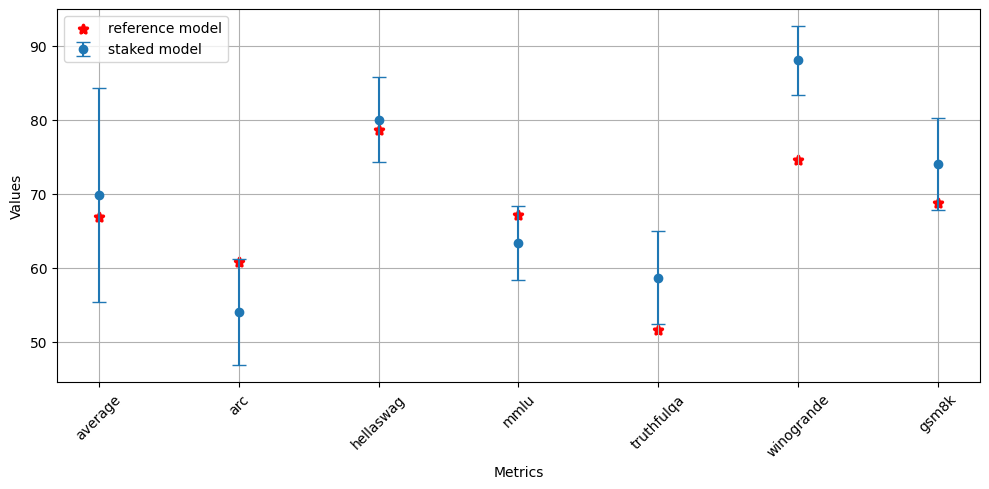
\includegraphics[width=0.8\textwidth]{llama3}
    \caption{Model: Llama-3-8b-instruct; Correlation Coef: 0.833 ; P-value: 0.039}
    \label{secb:fig:m1}
\end{figure}

\begin{figure}[htb!]
    \centering
    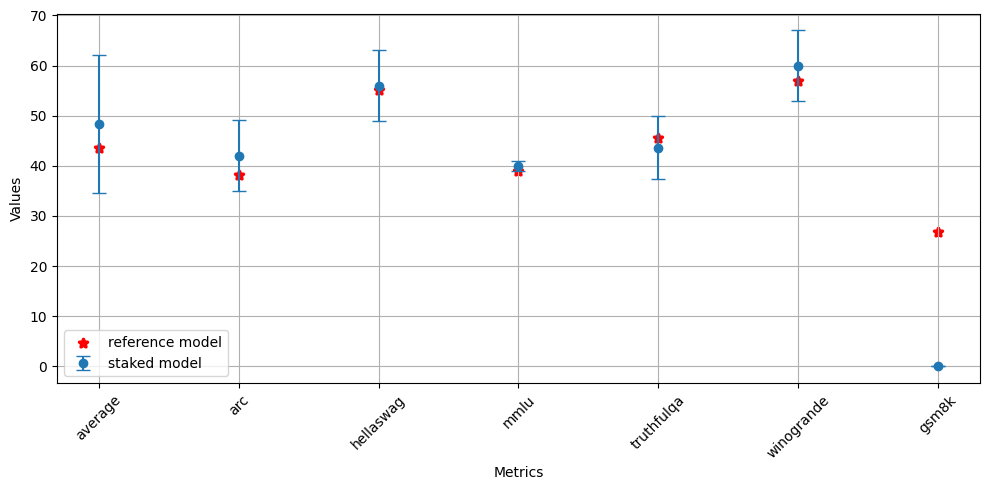
\includegraphics[width=0.8\textwidth]{deepseek}
    \caption{Model: Deepseek-coder-6.7B-instruct; Correlation Coef: 0.924 ; P-value: 0.009}
    \label{secb:fig:m2}
\end{figure}

\begin{figure}[htb!]
    \centering
    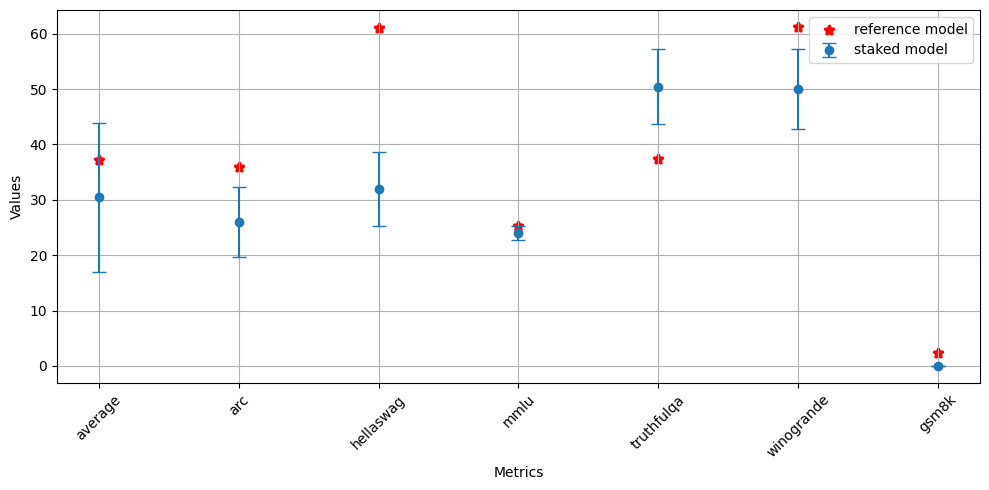
\includegraphics[width=0.8\textwidth]{tiny}
    \caption{Model: TinyLlama-1.1B-Chat-v1.0; Correlation Coef: 0.785 ; P-value: 0.064}
    \label{secb:fig:m3}
\end{figure}



\subsection{Conclusions}

The \gls{MLTB} was developed to perform arbitrary tests on \gls{ML} models that are staked in the POKT Network. 
In this first iteration it was configured to recreate the \gls{HFOLML}, a known source for model quality in the \gls{ML} community. 
After the initial tests we can say that the \gls{MLTB} is able to deliver on its promises: it was successfully deployed on a POKT Network local net, communicated with POKT nodes hosting \glspl{LM} and successfully retrieved the required data to populate the leaderboard. 

The \gls{MLTB} is not only able to reproduce the \gls{HFOLML} data, it also does it with much less samples (and hence cost) and keep high correlation with fully-sampled tests. 
Also, the test bench is created to be fully modular and scalable, being able to process tests form many nodes concurretly, something beyond the capabilities of the \gls{LMEH} that was not created to support loads as the ones we expect in the POKT Network. 

Regarding the update in the \gls{HFOLML}, it is important to recall what Borges said: "Thinking, analyzing, inventing are not anomalous acts, they are the normal breathing of intelligence". 
As the \gls{ML} field progresses, the adoption and refinement of frameworks like the \gls{LMEH} will remain crucial, ensuring that benchmarks evolve in tandem with the technologies they aim to measure. 
In the context of the POKT network, \gls{MLTB} is a first step towards the adoption of a decentralized \gls{ML} market following the state of the art in the field of benchmarking, and thus trying to shed light on the quality of service expected.
\section{Future Work}\label{sec:z}

hablar de que pokt-square no lo vamos a seguir laburando activamente.

decir cuales son las cosas que siguen en desarrollo

dar panorama para cuando primer mvp?
\newpage


%----------------------------------------------------------------------------------------
%	 Acronyms
%----------------------------------------------------------------------------------------
\printglossary[type=\acronymtype,title=List of Acronyms]

%----------------------------------------------------------------------------------------
%	 REFERENCES/BIBLIOGRAPHY
%----------------------------------------------------------------------------------------

\newpage

\addcontentsline{toc}{section}{Reference List} % Add the bibliography to the table of contents

%\begin{twothirdswidth} % Content in this environment to be at two-thirds of the whole page width
	\printbibliography[title=Reference List] % Output the bibliography with a custom section title
%\end{twothirdswidth}


%----------------------------------------------------------------------------------------

\end{document}	


